\section{Giới thiệu}
\label{sec:gioithieu}

Giao diện não--máy tính (brain--computer interface, BCI) chuyển hoạt động
điện não thành tín hiệu điều khiển cho thiết bị bên ngoài mà không đi qua
đường dẫn thần kinh--cơ thông thường \cite{chen2025brain, tonin2021noninvasive,
ding2026brain}. Phạm vi ứng dụng đã mở rộng từ phòng thí nghiệm sang các hệ
thống thực tế \cite{varbu2022present, pang2024applications} như xe lăn điện
\cite{palumbo2021motorimagery, lei2022intention, mai2024hybrid}, tay máy hỗ
trợ và chi giả \cite{casey2021bci}, thiết bị phục hồi chức năng chi trên
\cite{baniqued2021brain} và phương tiện di chuyển vận hành bằng ý định
\cite{lu2020model}. Nghiên cứu này tập trung vào tưởng tượng vận động
(motor imagery, MI), mô hình tín hiệu phù hợp với điều khiển chủ động kéo
dài do không cần kích thích ngoại vi \cite{palumbo2021motorimagery}. Trong
các hệ thống đó, bộ giải mã EEG là một khâu của vòng điều khiển kín. Thời
gian suy luận phải nằm trong ngân sách thời gian của vòng kín
\cite{an2024development, tonin2020role}. Mô hình phải chạy trên phần cứng
nhúng đi kèm thiết bị, nơi thời gian, bộ nhớ và năng lượng cần được xét
đồng thời \cite{sun2025signal, akbari2025atrial, craighero2024ondevice,
wang2024mibminet, pacini2024design, sen2025lowlatency}. Độ tin cậy phải ổn định giữa các phiên và giữa các đối
tượng, nhất là khi BCI chia sẻ quyền điều khiển với cơ chế tự hành
\cite{choi2023asynchronous, deng2020selfadaptive, wei2023intra}. Xu hướng
dùng thiết bị phổ thông ít kênh còn làm chất lượng tín hiệu giảm thêm
\cite{wu2022deepbrain, tarara2025motor, paneru2025eeg}. Bài báo dùng tốc độ
truyền thông tin (information transfer rate, ITR) \cite{wolpaw2002brain} và
ngân sách thời gian của vòng kín làm tiêu chí đánh giá bên cạnh độ chính xác
(Mục~\ref{sec:rangbuoc}).

Các yêu cầu này đặt người thiết kế bộ giải mã tưởng tượng vận động trước mâu thuẫn giữa độ chính xác và khả năng triển khai. Học sâu đã cải
thiện đáng kể chất lượng giải mã tưởng tượng vận động so với đặc trưng thủ
công \cite{al-saegh2021deep, sadiq2021development}. Các kiến trúc gọn nhẹ
như EEGNet \cite{lawhern2018eegnet} và các biến thể của nó
\cite{ingolfsson2020eegtcnet, deng2021advanced, wang2022mieeg,
wang2023ifnet} triển khai được trên phần cứng nhúng. Các mô hình dung lượng lớn hơn trải từ mạng tích chập sâu
\cite{schirrmeister2017deep}, transformer và kiến trúc lai
\cite{vafaei2025transformers, zhao2024ctnet, ding2025eegdeformer,
altaheri2025temporal, wang20232d} đến mô hình tập hợp nhiều thành phần
\cite{zoumpourlis2024motor}. Chúng chính xác hơn nhưng tốn kém khi suy luận
và phụ thuộc mạnh vào lượng dữ liệu huấn luyện \cite{keutayeva2024data,
keutayeva2024compact}. Chưng cất tri thức (knowledge distillation, KD) nhắm
trực tiếp vào mâu thuẫn này bằng cách truyền tri thức từ một teacher lớn
sang một student nhỏ mà không tăng chi phí suy luận của student
\cite{hinton2015distilling}. KD hiện là một trong những chiến lược chính để
xây dựng bộ giải mã EEG gọn nhẹ \cite{li2025lightweight, zhou2026structural},
bên cạnh tỉa trọng số, lượng tử hóa và tăng tốc phần cứng
\cite{xie2024comprehensive}.

Hai khoảng trống làm hạn chế giá trị của các so sánh cơ chế chưng cất hiện
có cho EEG. Khoảng trống đầu tiên nằm ở cách các cơ chế chưng cất được so sánh với nhau. Huấn luyện mạng sâu
chịu ảnh hưởng của nhiều nguồn ngẫu nhiên và ảnh hưởng này có thể lớn hơn
trên dữ liệu EEG vốn biến thiên mạnh giữa các đối tượng lẫn trong cùng một
đối tượng \cite{huang2023discrepancy}. Riêng việc đổi hạt giống ngẫu nhiên
đã có thể tạo chênh lệch đáng kể giữa các lần huấn luyện cùng một kiến trúc
\cite{picard2021torch}. So sánh phương pháp học máy cần tính đến các nguồn
biến thiên này \cite{bouthillier2021accounting} và lo ngại tương tự đã được
nêu cho học sâu trên dữ liệu thần kinh \cite{delpup2024toward}. Tuy vậy, so
sánh giữa các cơ chế chưng cất cho EEG vẫn thường được báo cáo từ một lần
chạy. Mức độ mà xếp hạng từ một lần chạy phản ánh khác biệt thật hầu như
chưa được đo trực tiếp. Khoảng trống còn lại nằm ở chính cách thiết kế các cơ chế chưng cất quan hệ. Ở các công trình hiện có, không gian đo quan hệ và cách chọn
cặp mẫu luôn thay đổi cùng nhau. Do đó không thể biết hiệu quả quan sát được
đến từ không gian biểu diễn hay từ cách tổ chức quan hệ.

Các phương pháp chưng cất được phân theo dạng tri thức truyền đi thành nhóm
dựa trên đầu ra, dựa trên đặc trưng và dựa trên quan hệ giữa các mẫu
\cite{gou2021knowledge, mansourian2025comprehensive}. Nhóm dựa trên đặc
trưng dùng gợi ý từ các tầng ẩn \cite{romero2015fitnets} và đã được áp dụng
cho ảnh y sinh \cite{javed2023knowledge}. Nhóm dựa trên quan hệ biểu diễn
tri thức bằng khoảng cách và góc giữa các vector biểu diễn
\cite{park2019relational}, độ tương đồng theo cặp \cite{feng2021double},
quan hệ trong lân cận cục bộ \cite{gou2025neighborhood} hoặc quan hệ xây
dựng đệ quy \cite{ye2021unsupervised}. Các nhóm này đã được mở rộng sang tự chưng cất
\cite{zhang2022selfdistillation, mai2025eegskdnet} và sang tín hiệu sinh lý
\cite{wang2021fldnet, gu2023framelevel, zhang2023distilling,
ibrahim2022knowledge, garcia-salinas2023intrasubject}. Với EEG, quan hệ giữa các mẫu tỏ ra đặc biệt phù hợp vì thông tin phân
biệt thường nằm ở cấu trúc tương đối giữa các mẫu. Similarity-Keeping Knowledge Distillation bảo toàn cấu trúc tương đồng
khi chuyển sang hệ thống ít điện cực \cite{huang2024enhancing}. Các khung
chưng cất nhiều mức đã được đề xuất cho tưởng tượng vận động
\cite{wu2026multilevel} và teacher dạng tập hợp đã được chưng cất thành một
backbone duy nhất dưới ràng buộc độ trễ \cite{xu2026entropy}. Ở các công trình này, cặp mẫu dùng để dựng quan hệ
phần lớn được chọn theo kinh nghiệm và quan hệ luôn được đo trong không gian
metric cổ điển.

Học máy lượng tử cung cấp một không gian đo quan hệ khác về bản chất. Một
mạch lượng tử tham số ánh xạ dữ liệu vào không gian Hilbert, trong đó tích
vô hướng giữa hai trạng thái đóng vai trò hàm nhân \cite{schuld2019quantum,
schuld2020circuitcentric, jerbi2023quantum}. Hàm nhân khó tính bằng máy cổ
điển không tự hàm ý lợi thế khi học \cite{huang2021power}. Hiệu quả của hàm nhân lượng tử còn phụ thuộc mạnh vào feature map và các
siêu tham số của nó \cite{jha2026comparative}. Khả năng khai thác các hàm
nhân này còn bị giới hạn bởi số qubit, độ sâu mạch và nhiễu của phần cứng
hiện nay \cite{xie2025advances, alam2022qnet}. Trong y sinh và EEG, thành phần lượng tử thường được chèn vào backbone
hoặc đặt ở cuối chuỗi xử lý \cite{idzikowski2026survey, chen2026exploring,
olvera2024eegbased, behera2026qsvmqnn, dutta2026duoqepinet}. Các thiết kế ở
lĩnh vực khác cũng theo cùng mẫu này
\cite{wang2022development, griol-barres2021variational, qi2024qtnvqc}.

Chưng cất tri thức lượng tử đã được dùng để nén mạng lượng tử
\cite{yan2026distilling} và đồng bộ các mô hình lượng tử phân tán
\cite{oh2025quantum}. Nó cũng đã được dùng để truyền tri thức từ teacher cổ
điển sang student lượng tử \cite{nishan2026quantummedkd,
barbato2026quantum} và giúp mạng cổ điển mô phỏng động lực học lượng tử
\cite{yao2023emulating}. Ở hướng nén và hướng student lượng tử, thành phần
lượng tử vẫn có mặt trong mô hình suy luận. Giống các thiết kế EEG nêu trên,
mô hình triển khai khi đó phải truy cập phần cứng lượng tử hoặc bộ mô phỏng lúc
chạy, mâu thuẫn với ràng buộc về độ trễ và tài nguyên. Quantum Relational
Knowledge Distillation (QRKD) và Quantum-Train chỉ dùng mạch lượng tử khi huấn luyện \cite{liu2025quantum,
liu2025quantumtrain}. Tiền đề của hướng này là hàm nhân lượng tử mô tả quan
hệ giữa các biểu diễn theo cách khác hàm nhân cổ điển
\cite{liu2022representation}. Cách làm này phù hợp với một bộ
giải mã trong vòng điều khiển nhưng QRKD mới được kiểm chứng trên thị giác
và ngôn ngữ với một cấu trúc quan hệ cố định.

Bảng~\ref{tab:sosanhcongtrinh} so sánh nghiên cứu này với các công trình
chưng cất quan hệ gần nhất theo dữ liệu, không gian đo quan hệ, cách chọn cặp
mẫu và việc dùng thành phần lượng tử khi suy luận.

\begin{table}[!htbp]
\centering
\caption{So sánh nghiên cứu này với các công trình chưng cất quan hệ gần nhất.}
\label{tab:sosanhcongtrinh}
\small
\begin{tabular}{>{\raggedright\arraybackslash}p{3.0cm}>{\raggedright\arraybackslash}p{2.8cm}>{\raggedright\arraybackslash}p{2.6cm}>{\raggedright\arraybackslash}p{2.8cm}>{\raggedright\arraybackslash}p{1.9cm}}
\toprule
\textbf{Công trình} & \textbf{Dữ liệu} & \textbf{Không gian đo quan hệ} & \textbf{Cách chọn cặp mẫu} & \textbf{Lượng tử khi suy luận} \\
\midrule
SKD \cite{huang2024enhancing} & EEG, mật độ điện cực cao sang thấp & Euclid (đặc trưng) & Cố định & Không \\
Chưng cất nhiều mức \cite{wu2026multilevel} & EEG tưởng tượng vận động & Cổ điển & Không phải đối tượng khảo sát & Không \\
QRKD \cite{liu2025quantum} & Thị giác, ngôn ngữ & Hilbert (hàm nhân lượng tử) & Cố định & Không \\
Nghiên cứu này & EEG tưởng tượng vận động (PhysionetMI, Cho2017) & Cosine, RBF, hàm nhân lượng tử & Năm chiến lược, là biến khảo sát & Không \\
\bottomrule
\end{tabular}
\end{table}

Nghiên cứu này xây dựng một khung chưng cất quan hệ có cấu trúc (QRD) để
lấp hai khoảng trống trên trong điều kiện kiểm soát chặt. Khung QRD coi
chiến lược hình thành quan hệ và không gian đo tương đồng là hai trục thiết
kế riêng biệt và thay đổi lần lượt từng trục. Tương tác giữa hai trục được
kiểm riêng bằng một thí nghiệm giai thừa. Năm chiến lược quan hệ được khảo sát, trải từ quan hệ dày đặc, quan hệ thưa
dựa trên mẫu đại diện đến lựa chọn theo mức bất định của teacher. Chúng được
kết hợp với hàm nhân cosine, RBF và lượng tử trên cùng một hàm mất mát, mọi
thành phần khác giữ nguyên. Hàm nhân lượng tử không
được đưa vào như một giải pháp đề xuất. Nó là ca kiểm chứng khắt khe nhất
do hình học của không gian Hilbert không quy được về khoảng cách Euclid
trong không gian đặc trưng ban đầu. Mọi hàm nhân quan hệ chỉ tham gia tính
hàm mất mát nên mô hình đưa vào vòng điều khiển vẫn là một mạng cổ điển gọn
nhẹ.

Đóng góp của nghiên cứu là một giao thức đánh giá có kiểm soát cho các cơ
chế chưng cất trên EEG tưởng tượng vận động, cùng bằng chứng định lượng
rằng nhiễu do hạt giống ngẫu nhiên vượt khác biệt giữa các cơ chế. Cụ thể gồm ba nội dung sau, xếp theo mức độ quan trọng.

\begin{itemize}
\item Đóng góp chính là bằng chứng về bất ổn định theo hạt giống. Bằng chứng này
thu được bằng giao thức lấy đối tượng làm đơn vị thống kê, năm hạt giống cố
định và kế hoạch thống kê chốt trước khi chạy. Nhiễu hạt giống (khoảng 0,75
điểm phần trăm) lớn hơn khác biệt giữa các cơ chế (khoảng 0,46 điểm). Xếp
hạng từ một lần chạy hầu như không tương quan với xếp hạng trên năm hạt
giống (hệ số Spearman 0,14).

\item Khung QRD là môi trường kiểm chứng có kiểm soát cho bằng chứng trên.
Trong khung này, chưng cất mang lại lợi ích ổn định trên PhysionetMI và
Cho2017. Tuy nhiên không biến thể quan hệ hay hàm nhân nào, kể cả hàm nhân
lượng tử, tách khỏi đường cơ sở KDBase ở mức ý nghĩa thống kê.

\item Mọi cấu hình được đánh giá thêm theo hướng điều khiển, bằng ITR, ngân
sách thời gian suy luận và phép đo thời gian suy luận thật trên phần cứng
nhúng.
\end{itemize}

Phần còn lại của bài báo được tổ chức như sau. Mục~\ref{sec:phuongphap}
trình bày quy trình nghiên cứu, khung QRD cùng các biến thể và giao thức
đánh giá. Mục~\ref{sec:ketqua} trình bày và thảo luận kết quả, còn
Mục~\ref{sec:ketluan} kết luận và nêu hướng phát triển. Chi tiết cài đặt,
các phép đối chứng bổ sung và bảng số liệu đầy đủ được đặt ở phụ lục.

\section{Phương pháp}
\label{sec:phuongphap}

\subsection{Quy trình nghiên cứu và tổng quan khung QRD}
\label{sec:tongquan}

Hình~\ref{fig:quytrinh} tóm tắt quy trình nghiên cứu, từ dữ liệu đến kết
luận thống kê. Bước đầu tiền xử lý tín hiệu và chia 103 đối tượng của
PhysionetMI thành năm fold theo một quy tắc tất định, không phụ thuộc hạt
giống (Mục~\ref{sec:dulieu}). Teacher sau đó được huấn luyện một lần cho
mỗi fold rồi giữ cố định. Với mỗi tổ hợp hạt giống, fold và cấu hình chưng
cất, student được huấn luyện và chọn checkpoint theo độ chính xác trên tập
kiểm định. Kết quả theo đối tượng được gộp thành một giá trị cho mỗi hạt
giống trước khi kiểm định theo kế hoạch chốt trước. Cuối cùng, cùng quy
trình được tái lập khám phá trên Cho2017 và student được đo thời gian suy
luận trên Raspberry Pi 4. Mục~\ref{sec:pipeline} trình bày quy trình này
dưới dạng giả mã (Thuật toán~2). Phần còn lại của mục này tập trung vào
khung QRD, tức khối cấu hình $c$ và nhánh QRD trong Hình~\ref{fig:quytrinh}.

\begin{figure}[H]
\centering
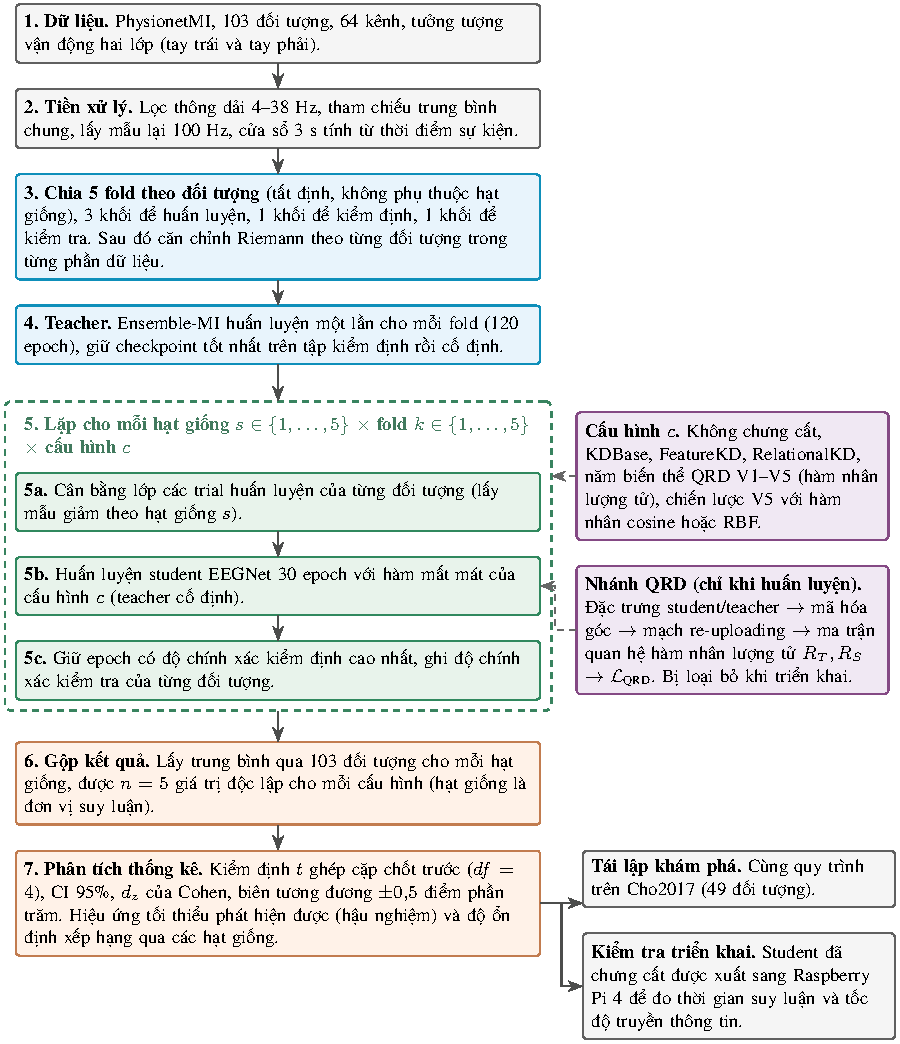
\includegraphics[width=0.92\linewidth]{figs/fig0_flow.pdf}
\caption{Quy trình nghiên cứu, từ dữ liệu đến phân tích thống kê. Khung nét
đứt là vòng lặp theo hạt giống, fold và cấu hình. Nhánh QRD chỉ có trong
giai đoạn huấn luyện.}
\label{fig:quytrinh}
\end{figure}
\FloatBarrier

Mục này mô tả cách các thành phần của khung QRD ghép nối với nhau và xác
định vai trò của từng thành phần trong quá trình huấn luyện.
Hình~\ref{fig:khung} thể hiện toàn bộ kiến trúc.

Khung được tổ chức theo thiết lập teacher--student. Teacher là một mô hình
tập hợp đã huấn luyện trước \cite{zoumpourlis2024motor}, được giữ cố định
và chỉ đóng vai trò nguồn tín hiệu giám sát. Student là một mạng EEGNet
\cite{lawhern2018eegnet} và là thành phần duy nhất trong cặp teacher--student
được cập nhật tham số \cite{hinton2015distilling}. Điểm ngoại lệ liên quan
đến mạch lượng tử dùng chung giữa hai nhánh được nêu ở Mục~\ref{sec:qrd}.

Cặp mô hình này được chọn để hiện thực hóa đúng mâu thuẫn đã nêu ở trên.
Mô hình tập hợp tổng hợp thông tin từ nhiều
thành phần nên cho tín hiệu giám sát ổn định. Nhưng chi phí bộ nhớ và tính
toán của nó tăng theo số thành phần, khiến nó kém phù hợp với phần cứng
nhúng đi kèm thiết bị. EEGNet ở chiều ngược lại có số tham số và thời gian suy luận phù hợp
với phần cứng nhúng và đã được kiểm chứng trong các hệ thống BCI triển
khai thực tế \cite{wang2024mibminet}. Khoảng cách hiệu năng giữa hai mô
hình chính là đại lượng mà khung chưng cất tìm cách thu hẹp.

Tín hiệu giám sát truyền tới student gồm thành phần khớp phân bố dự đoán mềm ở mức logits làm nền. Tùy cấu hình, nhiều nhất một trong ba thành phần bổ sung được cộng thêm. Hàm mất mát tổng quát cho cách kết hợp này được viết ở
\eqref{eq:total}, với hệ số của các thành phần không thuộc cấu hình đang
xét được đặt bằng không. Hai thành phần bổ sung đầu thuộc về chưng cất cổ
điển, gồm căn chỉnh đặc trưng trung gian và bảo toàn cấu trúc hình học
giữa các mẫu trong không gian đặc trưng. Cả hai được trình bày ở
Mục~\ref{sec:cocdien} và dùng làm cơ sở so sánh.

Thành phần bổ sung còn lại là nhánh quan hệ lượng tử, thành phần do nghiên cứu này bổ sung. Nhánh này nhận đặc trưng trung gian của cả hai mô hình, dựng ma trận
quan hệ trong không gian Hilbert và sinh ra một thành phần mất mát bổ
sung. Nó chỉ tồn tại trong đồ thị tính toán của giai đoạn huấn luyện, không
xuất hiện ở đường suy luận nên không làm thay đổi cấu hình của mô hình
được triển khai.

\begin{figure}[H]
\centering
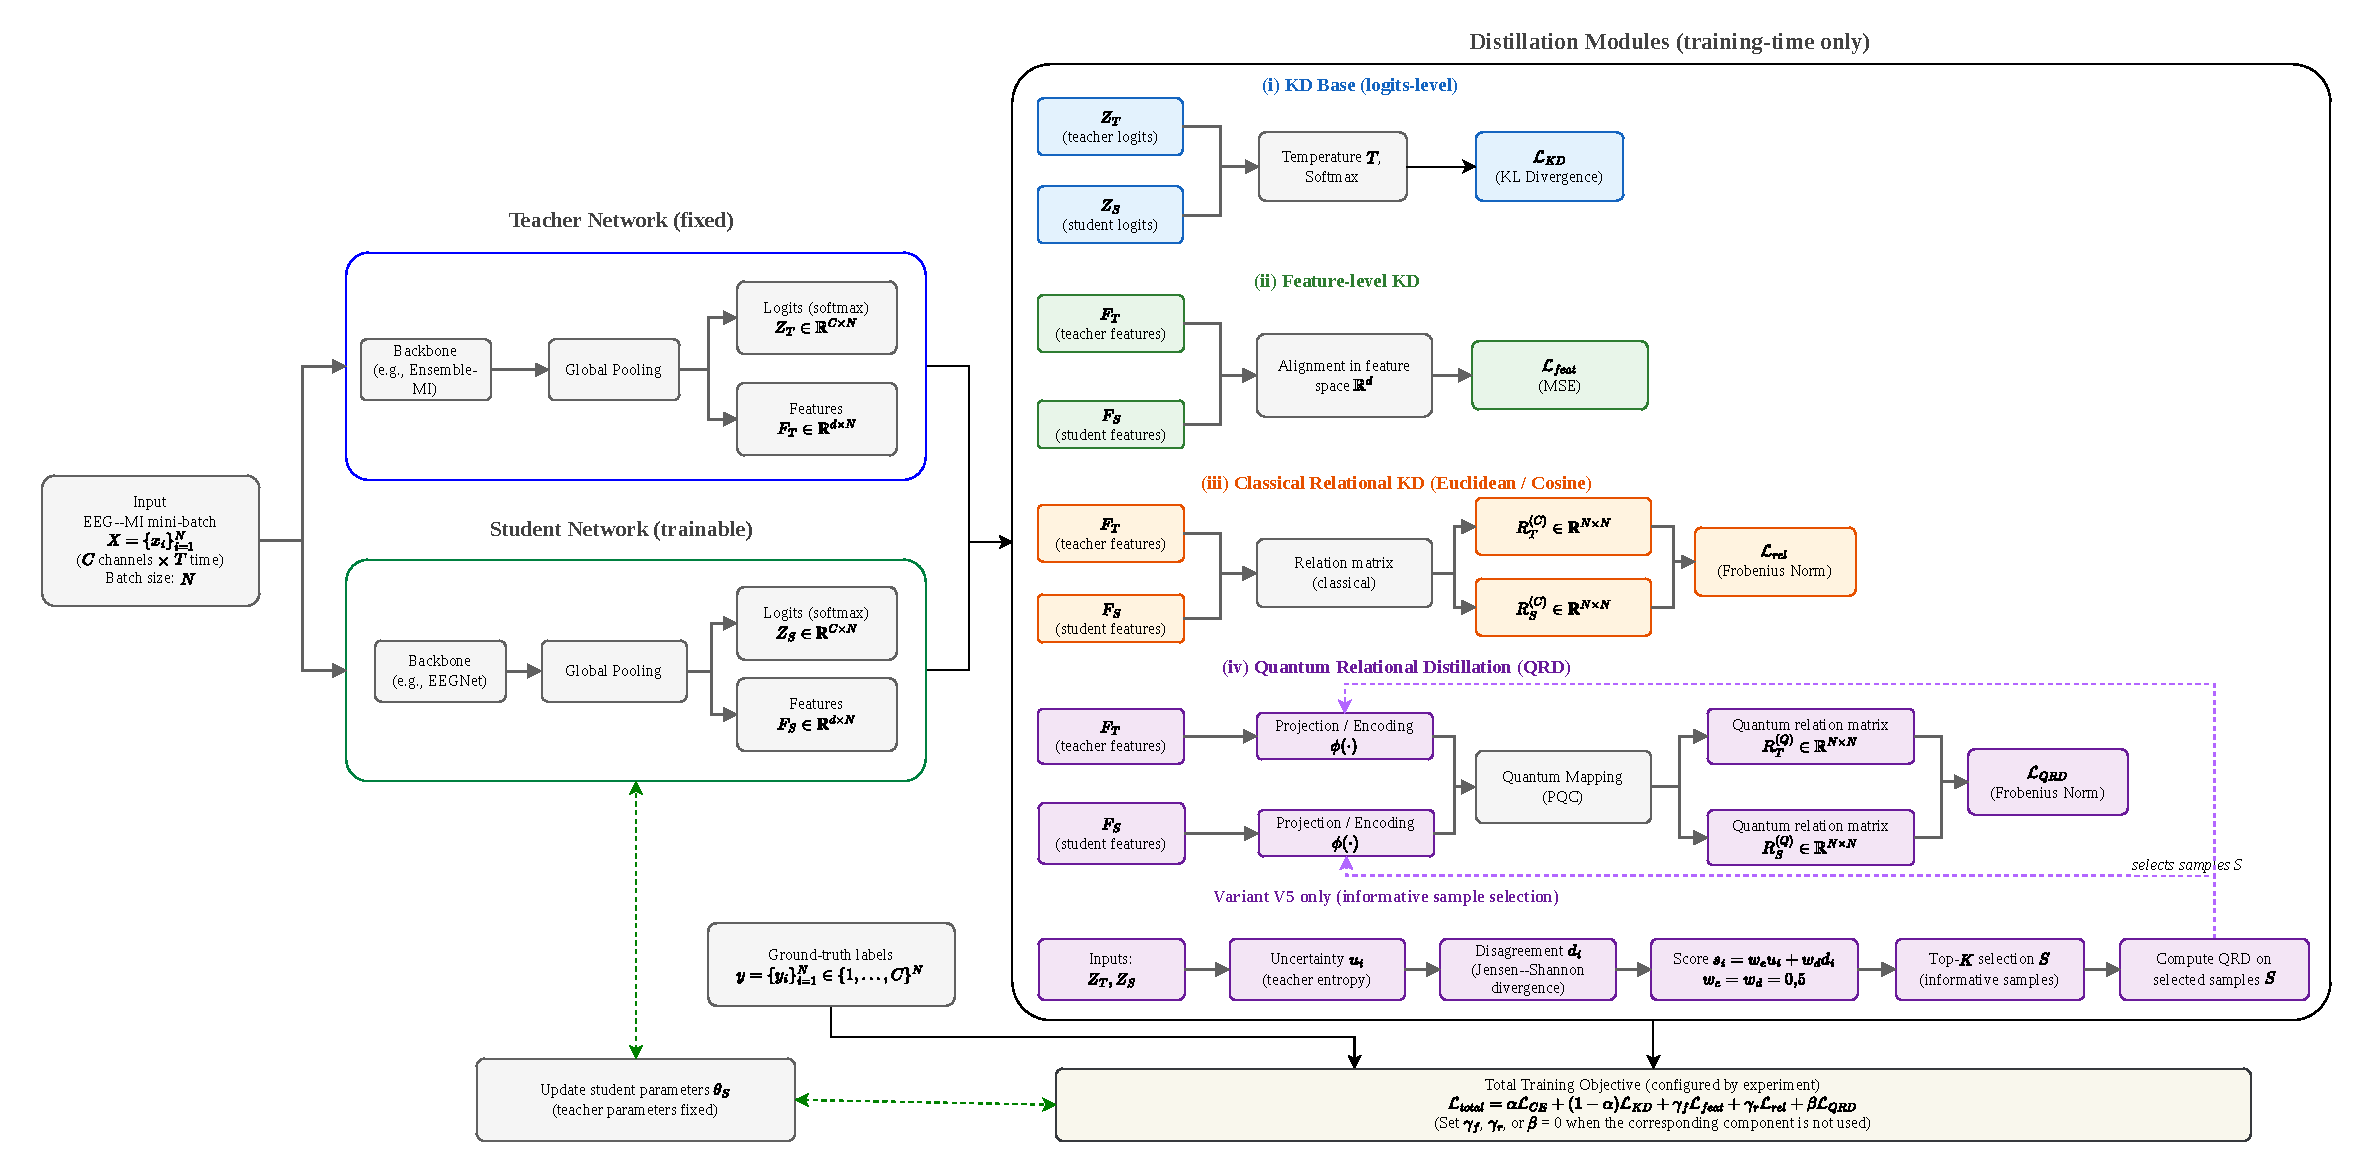
\includegraphics[width=\linewidth]{figs/fig12_QRD.drawio.pdf}
\caption{Khung teacher--student tổng thể với nhánh chưng cất quan hệ
lượng tử đề xuất.}
\label{fig:khung}
\end{figure}
\FloatBarrier

Phần còn lại của mục này quy ước ký hiệu dùng thống nhất cho toàn bộ
Mục~\ref{sec:phuongphap}.
Xét một mini-batch gồm $N$ mẫu EEG $\{x_i\}_{i=1}^{N}$. Với mỗi mẫu, mỗi mô hình sinh ra hai dạng đầu ra. Đó là vector logits $z_T(x_i), z_S(x_i) \in \mathbb{R}^{C}$ ở tầng phân loại và vector đặc trưng $f_T(x_i), f_S(x_i) \in \mathbb{R}^{d}$ ở tầng biểu diễn cuối ngay trước tầng đó. Với cặp mô
hình được sử dụng, $C = 2$ và $d = 144$ cho cả teacher và student.

Xếp các vector đặc trưng theo cột cho ma trận đặc trưng của mini-batch, khớp
quy ước dùng trong Hình~\ref{fig:khung}:

\begin{equation}
\label{eq:featmat}
F_T = \begin{bmatrix} f_T(x_1) & \cdots & f_T(x_N) \end{bmatrix}
\in \mathbb{R}^{d \times N},
\qquad
F_S = \begin{bmatrix} f_S(x_1) & \cdots & f_S(x_N) \end{bmatrix}
\in \mathbb{R}^{d \times N}.
\end{equation}

Chưng cất ở mức quan hệ không so sánh trực tiếp $F_T$ với $F_S$ mà so sánh
cấu trúc quan hệ giữa các mẫu trong từng mô hình. Cấu trúc này được biểu diễn bằng hai ma trận đối xứng $R_T$ và $R_S$. Phần tử $(i,j)$ của mỗi ma trận đo mức tương đồng giữa hai mẫu $x_i$ và $x_j$ theo biểu diễn của mô hình tương ứng.
Trong các phương pháp chưng cất quan hệ cổ điển, hai ma trận này được xây
dựng từ khoảng cách Euclid hoặc độ tương đồng cosine trong không gian đặc
trưng \cite{park2019relational}. Mục~\ref{sec:qrd} thay không gian đó bằng một
không gian Hilbert, trong đó mức tương đồng được đo bằng hàm nhân lượng tử.

Ma trận quan hệ không nhất thiết được tính trên toàn bộ mini-batch. Tập cặp chỉ số tham gia, ký hiệu $\mathcal{I}$, là một tham số cấu hình và
được xác định riêng cho từng biến thể ở Mục~\ref{sec:bienthe}.

\subsection{Các thiết lập chưng cất cổ điển}
\label{sec:cocdien}

Mục này định nghĩa ba cấu hình chưng cất cổ điển được dùng làm đường cơ sở.
Cả ba chia sẻ chung teacher, student, bộ dữ liệu và giao thức tối ưu. Thành
phần duy nhất thay đổi là dạng tín hiệu giám sát bổ sung. Nhờ ràng buộc này,
khác biệt hiệu năng quan sát được đều quy về cơ chế truyền tri thức.

\textbf{KDBase} thực hiện chưng cất ở mức đầu ra, khớp phân bố dự đoán mềm
của student với của teacher thông qua phân kỳ Kullback--Leibler có làm mềm
nhiệt độ \cite{hinton2015distilling}:

\begin{equation}
\label{eq:kd}
\mathcal{L}_{\mathrm{KD}} = \tau^{2}\,
  \mathrm{KL}\!\left(
  \sigma\!\left(\tfrac{z_T}{\tau}\right) \,\middle\|\,
  \sigma\!\left(\tfrac{z_S}{\tau}\right)\right),
\end{equation}

trong đó $\sigma(\cdot)$ là hàm softmax và $\tau = 4{,}0$ là nhiệt độ làm
mềm. Hệ số $\tau^{2}$ giữ độ lớn gradient không phụ thuộc vào $\tau$.

\textbf{FeatureKD} bổ sung ràng buộc ở mức đặc trưng trung gian
\cite{romero2015fitnets}. Vì student và teacher có cùng số chiều đặc trưng,
ràng buộc được áp trực tiếp mà không cần lớp chiếu trung gian:

\begin{equation}
\label{eq:feat}
\mathcal{L}_{\mathrm{feat}} = \frac{1}{Nd}
  \left\| F_S - F_T \right\|_{F}^{2}.
\end{equation}

\textbf{RelationalKD} chuyển trọng tâm từ từng mẫu sang quan hệ giữa các
mẫu \cite{park2019relational}. Nghiên cứu sử dụng thành phần khoảng cách
theo cặp của phương pháp gốc. Với mỗi mô hình, ma trận khoảng cách Euclid
theo cặp được chuẩn hóa bằng giá trị trung bình của các phần tử ngoài đường
chéo:

\begin{equation}
\label{eq:pdist}
\tilde{D}_{ij} = \frac{\|f_i - f_j\|_2}
  {\dfrac{1}{N(N-1)}\displaystyle\sum_{p \neq q} \|f_p - f_q\|_2},
\end{equation}

và sai lệch giữa hai ma trận đã chuẩn hóa được đo bằng hàm Huber:

\begin{equation}
\label{eq:rkd}
\mathcal{L}_{\mathrm{rel}} = \ell_{\delta}\!\left(
  \tilde{D}^{S}, \tilde{D}^{T} \right),
\end{equation}

với $\ell_{\delta}$ là hàm mất mát smooth L1. Phép chuẩn hóa theo giá trị trung bình khiến hàm mất mát bất biến với phép co giãn đồng nhất của không gian đặc trưng. Nhờ đó student chỉ cần tái tạo cấu trúc tương đối của biểu diễn teacher chứ không phải độ lớn tuyệt đối.

Hàm mất mát tổng của một cấu hình bất kỳ có dạng

\begin{equation}
\label{eq:total}
\mathcal{L} = \alpha\,\mathcal{L}_{\mathrm{CE}}
  + (1-\alpha)\,\mathcal{L}_{\mathrm{KD}}
  + \gamma_{f}\,\mathcal{L}_{\mathrm{feat}}
  + \gamma_{r}\,\mathcal{L}_{\mathrm{rel}}
  + \beta\,\mathcal{L}_{\mathrm{QRD}},
\end{equation}

trong đó $\mathcal{L}_{\mathrm{CE}}$ là entropy chéo với nhãn thật và các
thành phần không thuộc cấu hình đang xét được đặt hệ số bằng không. Thành
phần $\mathcal{L}_{\mathrm{QRD}}$ được trình bày ở Mục~\ref{sec:qrd}. Giá
trị các hệ số được nêu ở Mục~\ref{sec:cauhinh}.

Ba cấu hình trên tạo thành một dãy tăng dần về mức trừu tượng của tri thức
được truyền, từ đầu ra đến đặc trưng riêng lẻ rồi đến quan hệ giữa các mẫu.
RelationalKD là cấu hình đầu tiên trong dãy biểu diễn tri thức dưới dạng
quan hệ và cũng là điểm mà khung QRD mở rộng. Thay vì đo quan hệ bằng
khoảng cách Euclid trong không gian đặc trưng, QRD đo chúng bằng hàm nhân
trong không gian Hilbert.

\subsection{Khung chưng cất quan hệ lượng tử}
\label{sec:qrd}

Hàm nhân lượng tử được đưa vào để mở rộng phạm vi của kết luận chứ không
phải như một giải pháp đề xuất (Mục~\ref{sec:gioithieu}). Các chiến lược
quan hệ cổ điển đều dựng cấu trúc trong cùng một không gian metric. Nếu chỉ
so sánh chúng với nhau, một kết quả âm có thể quy cho việc chưa thực sự thay
đổi không gian biểu diễn.

Nhánh quan hệ lượng tử gồm ba bước: giảm chiều và mã hóa đặc trưng thành
góc quay, chuẩn bị trạng thái lượng tử và tính hàm nhân để dựng ma trận
quan hệ.

\textbf{Giảm chiều và mã hóa góc.} Vector đặc trưng $d = 144$ chiều không thể
mã hóa trực tiếp vào một mạch $n_q = 4$ qubit. Mỗi mô hình được gán một phép
chiếu tuyến tính riêng $W_T, W_S : \mathbb{R}^{d} \to \mathbb{R}^{n_q}$. Phép
chiếu phía teacher $W_T$ được khởi tạo và \textbf{giữ cố định} trong suốt quá
trình huấn luyện. Chỉ phép chiếu phía student $W_S$ là tham số khả huấn duy
nhất trong hai phép chiếu này. Biến thể V1 ở Mục~\ref{sec:bienthe} thay $W_S$
bằng một phép giảm chiều tất định, khi đó nhánh lượng tử phía student cũng
không còn tham số học được ở bước chiếu.

Phép chiếu $W_T$ được khởi tạo trong cùng luồng số ngẫu nhiên toàn cục
nên nhiều khả năng khác nhau giữa các hạt giống. Ảnh hưởng của biến thiên
này được kiểm tra bằng một đối chứng cố định $W_T$
(Phụ lục~\ref{app:doichung}). Chi tiết khởi tạo và giới hạn lý thuyết của phép
chiếu nêu ở Phụ lục~\ref{app:caidat}. Đầu ra $Wf(x_i)$ của phép chiếu
không bị giới hạn về độ lớn, trong khi góc quay dùng cho cổng lượng tử
cần nằm trong một khoảng xác định. Vì vậy, đầu ra này được chặn về
khoảng góc hợp lệ bằng hàm tiếp tuyến hyperbol trước khi dùng làm góc
quay:

\begin{equation}
\label{eq:angles}
a(x_i) = \pi \, \tanh\!\big( W f(x_i) \big) \in [-\pi, \pi]^{n_q}.
\end{equation}

Phép chặn này giới hạn góc quay trong một chu kỳ đầy đủ, giảm nguy cơ hai
giá trị đặc trưng khác nhau ánh xạ vào cùng một trạng thái do tính tuần hoàn
của phép quay.

\textbf{Chuẩn bị trạng thái.} Vector góc được nạp vào mạch bằng phép mã hóa góc quanh trục $Y$, ký hiệu $\Phi(\cdot)$. Phép mã hóa xen kẽ với $L = 2$ lớp cổng vướng víu dạng Strongly Entangling Layers \cite{schuld2020circuitcentric}, ký hiệu $U(\theta_l)$ cho lớp thứ $l$. Khác với một mạch mã hóa-rồi-vướng víu một
lượt, mã hóa được lặp lại xen kẽ giữa các lớp vướng víu theo kiểu
\emph{data re-uploading} \cite{perezsalinas2020data}:

\begin{equation}
\label{eq:layer}
\ket{\varphi_l(x_i)} = U(\theta_l)\,\Phi\!\big(a(x_i)\big)\,\ket{\varphi_{l-1}(x_i)},
\qquad
\ket{\varphi_0(x_i)} = \ket{0}^{\otimes n_q},
\qquad l = 1,\ldots,L,
\end{equation}

\begin{equation}
\label{eq:state}
\ket{\psi(x_i)} = \Phi\!\big(a(x_i)\big)\,\ket{\varphi_L(x_i)}.
\end{equation}

Với $L=2$, chuỗi cổng đầy đủ là mã hóa--vướng víu--mã hóa--vướng víu--mã hóa.
Dữ liệu được nạp lại ba lần, xen kẽ với hai lớp vướng víu tham số hóa. Các
tham số $\theta = (\theta_1,\ldots,\theta_L)$ được khởi tạo một lần từ phân
bố chuẩn $\mathcal{N}(0, 0{,}1)$. Chúng \textbf{là tham số khả huấn}, cập nhật
qua lan truyền ngược cùng với $W_S$ trong suốt quá trình huấn luyện. Mạch
$U(\theta_l)$ dùng \textbf{chung một bộ $\theta$} cho cả nhánh teacher và
nhánh student mà không tách $\theta_T$/$\theta_S$ riêng. Hệ quả của lựa chọn
này với tính "cố định" của teacher được phân tích ở phần sau của mục này.

Việc huấn luyện $\theta$ chỉ có ý nghĩa nếu lớp vướng víu $U(\theta_l)$
thực sự ảnh hưởng tới hàm nhân chứ không tự triệt tiêu khỏi phép tính.
Rủi ro này có thật trong một mạch mã hóa-rồi-vướng víu một lượt,
$\ket{\psi(x_i)} = U_\theta\,\Phi(a(x_i))\,\ket{0}^{\otimes n_q}$, nơi lớp
vướng víu $U_\theta$ là toán tử \emph{giống nhau cho mọi mẫu} và nằm ngoài
cùng của biểu thức. Hàm nhân khi đó chỉ phụ thuộc tích vô hướng
$\braket{\psi(x_i)|\psi(x_j)} = \bra{0}\Phi(a(x_i))^\dagger U_\theta^\dagger U_\theta \Phi(a(x_j))\ket{0}$. Vì $U_\theta^\dagger U_\theta = I$ với mọi $\theta$, lớp vướng víu triệt tiêu hoàn toàn khỏi hàm nhân bất kể được huấn luyện thế nào và mạch suy biến về một hàm nhân cổ điển của riêng $\Phi$.

Cấu trúc data re-uploading ở \eqref{eq:layer}--\eqref{eq:state} tránh
được suy biến này. Phép mã hóa cuối cùng $\Phi(a(x_i))$ là toán tử
\emph{phụ thuộc mẫu} và nằm ngoài cùng thay cho $U_\theta$ nên không còn
phép rút gọn tương tự. $U(\theta_l)$ không thể tách khỏi tích vô hướng
bằng lập luận unita độc lập dữ liệu. Kiểm chứng thực nghiệm trên một batch cố định cho sai khác $0{,}474$ giữa hàm nhân lượng tử và tích cosine tương ứng (Phụ lục~\ref{app:caidat}). Mạch do đó không suy biến về hàm nhân cổ điển.

Mạch khi đó không còn là một ánh xạ đặc trưng ngẫu nhiên cố định vào không
gian Hilbert $2^{n_q}$ chiều như trong một thiết kế mã hóa một lượt mà là
một ánh xạ đặc trưng \emph{khả huấn}. Khả năng thích nghi với dữ liệu của
nhánh lượng tử nằm ở $W_S$ và $\theta$. $W_T$ vẫn cố định như đã nêu ở trên.

\textbf{Hàm nhân và ma trận quan hệ.} Mức tương đồng giữa hai mẫu được đo
bằng độ trung thực giữa hai trạng thái tương ứng \cite{schuld2019quantum}:

\begin{equation}
\label{eq:kernel}
K\!\big(a_i, a_j\big) =
  \big| \braket{ \psi(x_i) | \psi(x_j) } \big|^{2} \in [0,1].
\end{equation}

Áp dụng riêng cho từng mô hình thu được hai ma trận quan hệ lượng tử:

\begin{equation}
\label{eq:relmat}
R_T^{(Q)}(i,j) = K\!\big(a_T(x_i), a_T(x_j)\big),
\qquad
R_S^{(Q)}(i,j) = K\!\big(a_S(x_i), a_S(x_j)\big),
\end{equation}

trong đó $a_T$ và $a_S$ là vector góc thu được từ \eqref{eq:angles} với phép
chiếu tương ứng. Hai ma trận được sử dụng trực tiếp mà không qua bước chuẩn hóa
bổ sung vì hàm nhân đã nhận giá trị trong đoạn $[0,1]$ theo định nghĩa.

\textbf{Hàm mất mát.} Sai lệch giữa hai cấu trúc quan hệ được đo bằng sai số
bình phương trung bình trên tập cặp chỉ số $\mathcal{I}$:

\begin{equation}
\label{eq:qrd}
\mathcal{L}_{\mathrm{QRD}} = \frac{1}{|\mathcal{I}|}
  \sum_{(i,j) \in \mathcal{I}}
  \left( R_T^{(Q)}(i,j) - R_S^{(Q)}(i,j) \right)^{2}.
\end{equation}

Gradient được truyền qua mạch lượng tử tới phép chiếu $W_S$ và tiếp tục tới mạng student. Thành phần này do đó ảnh hưởng tới toàn bộ quá trình học của student chứ không chỉ tới lớp chiếu. Phép chiếu $W_T$ tham gia vào tính toán
$R_T^{(Q)}$ nhưng không nhận gradient, đúng như đã nêu ở trên.

Tuy nhiên $R_T^{(Q)}$ không hoàn toàn tĩnh. Việc tính $R_T^{(Q)}$ không được
tách khỏi đồ thị tính toán. Không có bước \texttt{detach} hay
\texttt{no\_grad} nào bao quanh nhánh teacher trong \eqref{eq:qrd} nên
gradient của $\mathcal{L}_{\mathrm{QRD}}$ vẫn truyền tới $\theta$ qua cả
nhánh teacher lẫn nhánh student. Backbone của teacher và phép chiếu $W_T$
giữ cố định nhưng ánh xạ từ đặc trưng teacher sang $R_T^{(Q)}$ vẫn thay đổi theo $\theta$ trong suốt quá trình huấn luyện. Ngược lại, ở các thiết lập chưng cất cổ điển của Mục~\ref{sec:cocdien}, mục tiêu teacher hoàn toàn cố định.

Về nguyên tắc, việc dùng chung $\theta$ mở ra một hướng tối ưu khác cho
\eqref{eq:qrd}. Quá trình huấn luyện có thể xê dịch $\theta$ để hai ma trận dễ khớp nhau hơn, ví dụ làm cả hai hàm nhân phẳng hơn. Khi đó student không còn bị buộc tái tạo đúng cấu trúc quan hệ mà teacher đã học. Đây là dạng suy
biến khác với suy biến hàm nhân cổ điển do triệt tiêu $U_\theta$ đã xét
ở trên. Tách $\theta_T$ cố định riêng khỏi $\theta_S$ khả huấn sẽ tránh được rủi ro này. Đổi lại, hai nhánh không còn được đo bằng cùng một hàm nhân, khiến việc so sánh trực tiếp $R_T^{(Q)}$ với $R_S^{(Q)}$ trong
\eqref{eq:qrd} mất căn cứ. Nghiên cứu này chọn dùng chung $\theta$ và
kiểm tra đánh đổi đó bằng đối chứng ở Phụ lục~\ref{app:doichung}.

Trong hàm mục tiêu tổng \eqref{eq:total}, các cấu hình QRD sử dụng
$\gamma_f = \gamma_r = 0$. Tức là student nhận đồng thời tín hiệu giám sát
từ nhãn thật, từ logits của teacher và từ cấu trúc quan hệ lượng tử. Hệ số $\beta$ nhỏ hơn hai bậc so với các hệ số còn lại. Lý do là $\mathcal{L}_{\mathrm{QRD}}$ là sai lệch giữa hai đại lượng bị chặn trong $[0,1]$ nên có độ lớn nhỏ hơn
nhiều so với các thành phần mất mát khác.

Cùng một $\beta = 0{,}02$ được dùng cho cả ba dạng hàm nhân so sánh ở
Mục~\ref{sec:bienthe} (lượng tử, cosine, RBF). Việc cả ba hàm nhân đều cho
giá trị trong $[0,1]$ chỉ đảm bảo thang đo của $\mathcal{L}_{\mathrm{QRD}}$
nằm trong cùng một khoảng. Nó không đảm bảo ba hàm nhân tạo ra cùng độ lớn gradient hay cùng mức ảnh hưởng lên student khi nhân với cùng một $\beta$.
RBF tự chuẩn theo trung vị khoảng cách của mỗi batch, còn hàm nhân lượng tử
có xu hướng tập trung giá trị gần biên do hình học không gian Hilbert.
Tổng quát hơn, phân bố giá trị của một hàm nhân lượng tử phụ thuộc mạnh
vào phép nhúng. Giá trị hàm nhân được biết là co cụm khi phép nhúng có
khả năng biểu đạt cao hơn \cite{thanasilp2024exponential}. Thang giá trị
hiệu dụng của nó do độ rộng hàm nhân (bandwidth) của phép mã hóa quyết
định \cite{shaydulin2022importance}. Mức chênh lệch độ lớn giám sát thực
tế giữa ba hàm nhân được đo và xử lý ở Mục~\ref{sec:chuyensau}.

\subsection{Các biến thể của khung QRD}
\label{sec:bienthe}

Năm biến thể được xây dựng trên cùng một hàm nhân lượng tử
\eqref{eq:kernel} và cùng một hàm mất mát \eqref{eq:qrd}. Chúng khác nhau ở cách đưa đặc trưng $d$ chiều xuống $n_q$ chiều trước khi mã hóa lượng tử. Chúng cũng khác nhau ở tập chỉ số $\mathcal{I}$ xác định những cặp mẫu nào tham gia vào ma trận quan hệ. Hình~\ref{fig:bienthe} minh họa năm thiết kế.

Thiết kế này xuất phát từ nhận xét rằng không phải mọi cặp mẫu đều mang lượng
thông tin như nhau. Tín hiệu EEG có tỷ lệ tín hiệu trên nhiễu thấp và biến
thiên mạnh giữa các đối tượng \cite{huang2023discrepancy} nên một ma trận
quan hệ dày đặc có thể chứa
nhiều cặp phản ánh nhiễu hơn là cấu trúc lớp.

\begin{figure}[H]
\centering
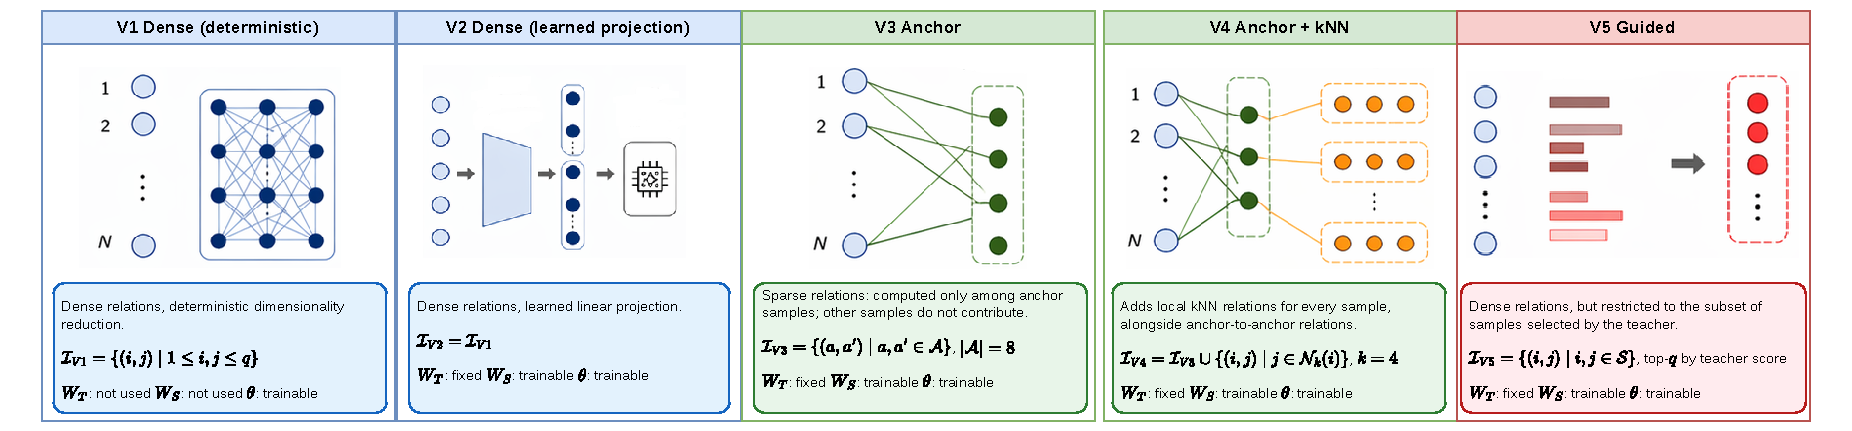
\includegraphics[width=\linewidth]{figs/fig2_QRD.pdf}
\caption{Năm biến thể của khung QRD.}
\label{fig:bienthe}
\end{figure}
\FloatBarrier

Bốn biến thể V1 đến V4 có chung một điểm cài đặt cần nêu trước. Chi phí mô phỏng mạch lượng tử tăng theo bình phương số mẫu. Ma trận quan hệ của bốn biến thể này do đó không được tính trên toàn bộ mini-batch kích thước $N$
mà trên một mẫu con \emph{cố định theo vị trí}. Mẫu con này gồm
$q = \min(16, N)$ phần tử đầu tiên của mỗi batch. Vì batch đã được xáo trộn ngẫu nhiên, mẫu con
này tương đương một phép lấy mẫu ngẫu nhiên không phụ thuộc nội dung. Mọi tập
chỉ số của V1 đến V4 dưới đây được hiểu là xác định trên $q$ mẫu đó.

\textbf{V1: quan hệ dày đặc, giảm chiều tất định.} Biến thể cơ sở không dùng
phép chiếu tuyến tính học được ở bước giảm chiều. Mạch lượng tử $\theta$ vẫn
được huấn luyện như mọi biến thể khác (Mục~\ref{sec:qrd}) nên biến thể này có 24 tham số bổ sung (chỉ $\theta$). Bốn biến thể còn lại có 604 tham số (580 từ $W_S$ cộng 24 từ $\theta$). Vector đặc trưng $d$ chiều
được chia đều thành $n_q$ nhóm liên tiếp, mỗi nhóm lấy trung bình:

\begin{equation}
\label{eq:chunk}
\big[g(f)\big]_m = \frac{n_q}{d}
  \sum_{l = (m-1)d/n_q + 1}^{m\,d/n_q} f_l,
  \qquad m = 1,\ldots,n_q,
\end{equation}

sau đó $g(f)$ thay cho $W f$ trong \eqref{eq:angles}. Tập chỉ số gồm toàn bộ
các cặp:

\begin{equation}
\label{eq:i-v1}
\mathcal{I}_{\mathrm{V1}} = \{(i,j) \mid 1 \le i,j \le q\}.
\end{equation}

Biến thể này là mở rộng
trực tiếp nhất của chưng cất quan hệ cổ điển sang không gian Hilbert và là
mốc so sánh cho bốn biến thể còn lại.

\textbf{V2: quan hệ dày đặc, phép chiếu học được.} Biến thể này giữ nguyên
tập chỉ số của V1 nhưng thay phép giảm chiều tất định bằng hai phép chiếu
tuyến tính $W_T$ và $W_S$ như mô tả ở Mục~\ref{sec:qrd}. Chỉ $W_S$ là tham số khả huấn, còn $W_T$ giữ cố định:

\begin{equation}
\label{eq:i-v2}
\mathcal{I}_{\mathrm{V2}} = \mathcal{I}_{\mathrm{V1}}.
\end{equation}

Cặp V1 và V2 so sánh hai thiết kế chiếu đặc trưng vào không gian góc. V1 dùng phép lấy trung bình cố định, không tham số, còn V2 dùng một cặp phép chiếu tuyến tính mà chỉ $W_S$ phía student được huấn luyện. So sánh
này đổi nhiều hơn là chỉ tính khả huấn của $W_S$. Chuyển từ V1 sang V2
cũng thay target của teacher từ trung bình theo khối tất định sang một
phép chiếu tuyến tính $W_T$ ngẫu nhiên (đông cứng). Việc khởi tạo thêm hai
lớp tuyến tính ở V2 còn tiêu thụ thêm số ngẫu nhiên so với phép lấy trung
bình không tham số của V1. So sánh V1 với V2 do đó nên được đọc là so sánh giữa hai thiết kế giảm chiều tổng thể. Đây không phải một đối chứng tách bạch riêng lợi ích hay chi phí của việc để $W_S$ khả huấn. Muốn kết luận nhân quả riêng
cho $W_S$ cần một đối chứng giữ cố định cả target phía teacher lẫn chuỗi số
ngẫu nhiên giữa hai biến thể.

\textbf{V3: quan hệ thưa dựa trên tập neo.} Để giảm mật độ quan hệ, biến thể
này giới hạn tập chỉ số trong một tập neo $\mathcal{A}$ có kích thước
$M = 8$:

\begin{equation}
\label{eq:i-v3}
\mathcal{I}_{\mathrm{V3}} = \{(a,a') \mid a, a' \in \mathcal{A}\},
\qquad \mathcal{A} \subset \{1,\ldots,q\}, \; |\mathcal{A}| = M.
\end{equation}

Tập neo là $M$ phần tử đầu của mẫu con. Thứ tự mẫu được xáo trộn lại ở
mỗi epoch nên đây là phép chọn ngẫu nhiên, không dựa trên nội dung mẫu. Lựa
chọn này có chủ ý, tách riêng ảnh hưởng của việc \emph{giảm mật độ} khỏi
ảnh hưởng của việc \emph{chọn có định hướng}, vốn được khảo sát ở V5. Các mẫu nằm ngoài $\mathcal{A}$ không đóng góp vào thành phần mất mát
quan hệ dù vẫn tham gia các thành phần khác của \eqref{eq:total}.

\textbf{V4: kết hợp quan hệ toàn cục và cục bộ.} Biến thể này bổ sung quan hệ
lân cận vào khối neo:

\begin{equation}
\label{eq:i-v4}
\mathcal{I}_{\mathrm{V4}} = \{(a,a') \mid a,a' \in \mathcal{A}\}
  \cup \{(i,j) \mid j \in \mathcal{N}_k(i)\},
\end{equation}

trong đó $\mathcal{N}_k(i)$ là tập $k = 4$ lân cận gần nhất của mẫu $x_i$.
Lân cận được xác định bằng khoảng cách Euclid trên đặc trưng của teacher, tức
là cấu trúc cục bộ được lấy từ mô hình đã huấn luyện chứ không từ student
đang học. Quan hệ thu được được đối xứng hóa. Nếu $j$ thuộc lân cận của $i$
thì cả hai cặp $(i,j)$ và $(j,i)$ đều thuộc $\mathcal{I}_{\mathrm{V4}}$. Khác
với V3, mọi mẫu trong mẫu con đều tham gia thông qua các cạnh lân cận của
mình. Vì $\mathcal{I}_{\mathrm{V4}}$ được định nghĩa như một tập hợp, một cặp
$(i,j)$ xuất hiện đồng thời trong khối neo lẫn khối kNN chỉ được tính đúng
một lần trong \eqref{eq:qrd} chứ không cộng dồn.

\textbf{V5: lựa chọn quan hệ có định hướng theo teacher.} Bốn biến thể trên
chọn mẫu không phụ thuộc nội dung, trên một tập con cố định $q$ phần tử. V5
thay tập con cố định đó bằng một tập con \emph{chọn theo nội dung}, với
candidate pool là toàn bộ $N$ mẫu của batch chứ không phải $q$ phần tử đầu.
Với mỗi mẫu $x_i$ trong toàn bộ batch ($i = 1,\ldots,N$), độ bất định của
teacher được đo bằng entropy chuẩn hóa của phân bố dự đoán:

\begin{equation}
\label{eq:entropy}
u_i = -\frac{1}{\log C}\sum_{c=1}^{C}
  p_T(c \mid x_i) \log p_T(c \mid x_i),
\end{equation}

với $C$ là số lớp, nhờ đó $u_i \in [0,1]$. Mức bất đồng thuận giữa teacher và
student được đo bằng phân kỳ Jensen--Shannon:

\begin{equation}
\label{eq:js}
d_i = \tfrac{1}{2}\mathrm{KL}\!\left(p_T \,\|\, m_i\right)
    + \tfrac{1}{2}\mathrm{KL}\!\left(p_S \,\|\, m_i\right),
\qquad m_i = \tfrac{1}{2}\left(p_T + p_S\right),
\end{equation}

trong đó $p_T$ và $p_S$ viết tắt cho $p_T(\cdot \mid x_i)$ và
$p_S(\cdot \mid x_i)$. So với chuẩn $L_2$, phân kỳ Jensen--Shannon có ưu điểm
là đối xứng, bị chặn và phù hợp với việc so sánh hai phân bố xác suất. Điểm
số tổng hợp là trung bình có trọng số của hai đại lượng, tính cho toàn bộ $N$
mẫu:

\begin{equation}
\label{eq:score}
s_i = w_e\,u_i + w_d\,d_i, \qquad w_e = w_d = 0{,}5,
\qquad i = 1,\ldots,N.
\end{equation}

Tập $\mathcal{S}$ gồm $q$ mẫu có điểm số cao nhất trong toàn bộ $N$ mẫu
được chọn. Ma trận quan hệ được dựng trên các cặp trong tập con kích thước
$q$ đó:

\begin{equation}
\label{eq:i-v5}
\mathcal{I}_{\mathrm{V5}} = \{(i,j) \mid i,j \in \mathcal{S}\},
\qquad \mathcal{S} = \operatorname*{arg\,top\text{-}q}_{i \in \{1,\ldots,N\}} s_i.
\end{equation}

Khác với V1--V4, nơi tập chỉ số $\mathcal{I}$ được xác định bằng vị trí cố
định hoặc đặc trưng đã đóng băng của teacher, phép chọn ở đây phụ thuộc dữ liệu. Tập $\mathcal{S}$ phụ thuộc điểm số $s_i$ qua một phép chọn rời rạc, không khả vi.
Trong khi đó, bước dựng ma trận quan hệ trên $\mathcal{S}$ vẫn cần lan
truyền ngược bình thường. Thuật toán~1 tóm tắt trình tự tính toán và làm rõ ranh
giới gradient giữa hai phần này.

\begin{quote}
\ttfamily\small\raggedright
\noindent\textbf{Thuật toán 1. Lựa chọn quan hệ theo teacher (V5).}\\[2pt]
\textbf{Vào:} logits teacher $Z_T \in \mathbb{R}^{C \times N}$, logits
student $Z_S \in \mathbb{R}^{C \times N}$, đặc trưng teacher/student
$F_T, F_S \in \mathbb{R}^{d \times N}$, kích thước tập chọn $q$.\\
\textbf{Ra:} ma trận quan hệ lượng tử $q \times q$ dùng cho
$\mathcal{L}_{\mathrm{QRD}}$.\\[4pt]
1: \quad \# Bước 1--3 nằm ngoài đồ thị gradient (torch.no\_grad)\\
2: \quad \textbf{với} $i = 1,\ldots,N$: tính $u_i$ theo \eqref{eq:entropy} từ
$Z_T$\\
3: \quad \textbf{với} $i = 1,\ldots,N$: tính $d_i$ theo \eqref{eq:js} từ
$Z_T, Z_S$\\
4: \quad \textbf{với} $i = 1,\ldots,N$: $s_i \leftarrow w_e u_i + w_d d_i$
(\eqref{eq:score})\\
5: \quad $\mathcal{S} \leftarrow$ chỉ số của $q$ giá trị $s_i$ lớn nhất trong
$N$ mẫu (\texttt{torch.topk}, không lan truyền ngược)\\[4pt]
6: \quad \# Từ đây gradient được nối lại bình thường\\
7: \quad $F_T[\mathcal{S}],\, F_S[\mathcal{S}] \leftarrow$ trích $q$ cột của
$F_T, F_S$ tại chỉ số $\mathcal{S}$\\
8: \quad Mã hóa $F_T[\mathcal{S}], F_S[\mathcal{S}]$ thành trạng thái lượng
tử theo \eqref{eq:angles}--\eqref{eq:state}\\
9: \quad Dựng $R_T^{(Q)}, R_S^{(Q)} \in \mathbb{R}^{q \times q}$ theo
\eqref{eq:kernel}--\eqref{eq:relmat} trên $q$ mẫu đã chọn\\
10: \quad Tính $\mathcal{L}_{\mathrm{QRD}}$ theo \eqref{eq:qrd} trên hai ma
trận $q \times q$ này
\end{quote}

Candidate pool ở dòng 2--4 là toàn bộ $N$ mẫu nên phép \texttt{top-q} ở
dòng 5 là một phép chọn thật sự, loại $N - q$ mẫu có điểm thấp. V1--V4 thì
không chọn gì sau khi đã cố định $q$ mẫu đầu theo vị trí. V5 vì vậy khác
V2--V4 ở cả tiêu chí chọn lẫn candidate pool. Thông tin ở mức đầu ra chỉ
định hướng việc chọn mẫu theo một quy tắc rời rạc, cố định theo
\eqref{eq:score}. Ma trận quan hệ vẫn được dựng từ đặc trưng trung gian và
tham gia đầy đủ vào lan truyền ngược (dòng 6--10).

Bảng~\ref{tab:bienthe_cauhinh} tóm tắt trạng thái huấn luyện của từng thành phần trong cả năm biến thể. Bảng giúp tránh nhầm lẫn giữa việc "không có phép chiếu học được" (V1) với việc "không có tham số học được nào", điều không đúng cho V1 vì mạch $\theta$ vẫn được huấn luyện. Cột tham số bổ sung không tính các
tham số của teacher/student vốn đã có sẵn ngoài nhánh QRD.

\begin{table}[!htbp]
\centering
\caption{Trạng thái huấn luyện của từng thành phần trong năm biến thể QRD.}
\label{tab:bienthe_cauhinh}
\small
\begin{tabular}{lccccc}
\toprule
\textbf{Biến thể} & $W_T$ & $W_S$ & $\theta$ & Tập cặp $\mathcal{I}$ & Tham số bổ sung \\
\midrule
V1 Dense (tất định) & không dùng & không dùng & huấn luyện & toàn bộ $q\times q$ & 24 \\
V2 Dense (chiếu học được) & cố định & huấn luyện & huấn luyện & toàn bộ $q\times q$ & 604 \\
V3 Anchor & cố định & huấn luyện & huấn luyện & neo $\mathcal{A}$, $M{=}8$ & 604 \\
V4 Anchor$+$kNN & cố định & huấn luyện & huấn luyện & neo $+$ kNN, $k{=}4$ & 604 \\
V5 Guided & cố định & huấn luyện & huấn luyện & top-$q$ theo teacher & 604 \\
\bottomrule
\end{tabular}
\end{table}
\FloatBarrier

Năm biến thể tạo thành hai trục khảo sát giao nhau. Trục đầu, gồm V1 và V2, xét khả năng thích nghi của phép giảm chiều. Trục sau, gồm V2 đến V5, xét mật độ và cách chọn quan hệ. Trục này đi từ không can thiệp, đến giảm mật độ ngẫu
nhiên, đến bổ sung cấu trúc cục bộ, rồi đến chọn mẫu theo nội dung. Song song
với hai trục này, việc thay hàm nhân lượng tử bằng hàm nhân cosine hoặc RBF
trong cùng một chiến lược tách riêng đóng góp của không gian biểu diễn.

\subsection{Dữ liệu, tiền xử lý và giao thức đánh giá}
\label{sec:dulieu}

Phương pháp được đánh giá trên bộ dữ liệu PhysioNet EEG Motor
Movement/Imagery \cite{schalk2004bci2000, goldberger2000physiobank}, gọi tắt
PhysionetMI theo tên lớp dữ liệu tương ứng trong MOABB. Bộ dữ liệu gồm bản
ghi điện não của 109 đối tượng thu bằng hệ thống 64 điện cực theo chuẩn
10--10 với tần số lấy mẫu 160 Hz. Theo danh sách loại trừ của công trình
teacher \cite{zoumpourlis2024motor}, sáu đối tượng có bản ghi không nhất
quán về thời lượng hoặc gán nhãn bị loại (mã số 88, 90, 92, 100, 104 và
106). Còn
lại 103 đối tượng được sử dụng.

Thực nghiệm tập trung vào bài toán hai lớp \emph{left\_hand} và
\emph{right\_hand}, paradigm hai lớp mặc định của lớp \texttt{PhysionetMI}
trong MOABB. Bài toán này phân biệt tưởng tượng nắm tay trái và nắm tay phải,
hai lệnh điều khiển cơ bản trong các hệ thống hỗ trợ vận hành bằng tín hiệu
não. Ba lớp còn lại của tập dữ liệu gốc (rest, feet,
hands) không được sử dụng. Số trial của mỗi đối tượng không cố định, dao
động theo số lần ghi thực tế còn giữ lại. Với mỗi đối tượng, các trial \emph{huấn luyện} được lấy mẫu giảm theo lớp
về đúng số lượng của lớp ít hơn, bằng lấy mẫu ngẫu nhiên không hoàn lại theo
hạt giống huấn luyện. Tập huấn luyện do đó cân bằng lớp theo từng đối tượng.
Hạt giống ngẫu nhiên vì thế còn chi phối việc trial huấn luyện nào được giữ
lại, ngoài khởi tạo trọng số và thứ tự batch. Tập kiểm định và tập kiểm tra
giữ nguyên mọi trial của các lớp đã chọn, không cân bằng lại.

Tín hiệu thô 160 Hz được xử lý qua bốn bước tuần tự. Tín hiệu được lọc
thông dải 4--38 Hz bằng bộ lọc FIR pha không theo cấu hình mặc định của
MNE/braindecode, không chỉnh bậc bộ lọc tường minh. Sau đó tín hiệu được tái
tham chiếu theo trung bình chung (Common Average Reference), lấy mẫu lại
xuống 100 Hz và cắt cửa sổ. Không có bước lọc
notch và không có bước loại artifact tường minh (không ICA, không ngưỡng loại
trial). Mỗi epoch bắt đầu đúng tại thời điểm sự kiện, không
có độ trễ offset đầu hay cuối và kéo dài 3,0 s, tương ứng 300 mẫu ở tần số 100 Hz sau khi lấy mẫu lại.

Sau khi cắt cửa sổ và chia tập huấn luyện, kiểm định và kiểm tra như mô tả ở dưới, một bước thứ
năm được áp dụng: căn chỉnh hiệp phương sai Riemannian, theo đúng cách cài
đặt của mã nguồn teacher \cite{zoumpourlis2024motor}. Hình học Riemannian
của ma trận hiệp phương sai được dùng rộng rãi trong học chuyển giao tưởng
tượng vận động chéo đối tượng nhằm xử lý biến thiên giữa các đối tượng
\cite{xu2021selective}. Với mỗi đối tượng, riêng trong từng tập huấn luyện, kiểm định và kiểm tra,
một ma trận hiệp phương sai không gian được ước lượng cho từng trial bằng bộ
ước lượng OAS. Các ma trận này được lấy trung bình Riemannian
(affine-invariant) qua các trial của đối tượng đó. Giá trị trung bình xác
định một phép biến đổi làm trắng ($\mathrm{cov}^{-1/2}$), được áp dụng lên
mọi trial của đối tượng đó trong tập tương ứng. Đây là bước duy nhất
ngoài quy đổi đơn vị có chạm vào cấu trúc biên độ/hiệp phương sai của tín
hiệu.

Bước căn chỉnh này có hệ quả trực tiếp tới cách diễn giải độ chính xác đã
báo cáo. Phép biến đổi làm trắng cho một đối tượng kiểm tra được ước lượng từ chính
các trial kiểm tra của đối tượng đó nên giao thức đánh giá là \emph{offline
và transductive ở mức đối tượng}. Việc căn chỉnh một trial kiểm tra dùng
thống kê bậc hai gộp trên toàn bộ trial kiểm tra của đối tượng đó. Trong một
triển khai ra lệnh trực tuyến, một số trial này sẽ chưa có sẵn tại thời điểm
suy luận. Bước này không trộn thông tin giữa các đối tượng và không dùng
\emph{nhãn} kiểm tra. Vì thế nó không phải rò rỉ huấn luyện/kiểm tra theo
nghĩa thông thường, tức khi bước tiền xử lý được khớp chung trên cả dữ liệu
huấn luyện và dữ liệu kiểm tra \cite{kapoor2023leakage}. Các con số độ chính
xác trong bài định lượng việc giải mã khi có sẵn một khối dữ liệu không nhãn
từ cùng phiên để căn chỉnh. Chúng không định lượng việc giải mã từng cửa sổ
đơn lẻ cho người dùng mới chưa có dữ liệu nào. Muốn khẳng định trực tiếp khả
năng triển khai trực tuyến hoặc inductive cần ước lượng phép biến đổi này
chỉ từ dữ liệu có sẵn trước mỗi lần suy luận. Ví dụ là một khối hiệu chỉnh
ghi ở đầu phiên hoặc một ước lượng trực tuyến cập nhật dần. Nghiên cứu này
chưa chạy giao thức như vậy. Phép đo độ trễ trên
Pi 4 ở Mục~\ref{sec:danhgiadk} chỉ đo thời gian forward của mạng,
chưa gồm chi phí ước lượng hay áp dụng bước căn chỉnh này.

Giao thức đánh giá là kiểm chéo 5-fold chia theo đối tượng nhằm bảo đảm không
đối tượng nào xuất hiện đồng thời ở tập huấn luyện và tập kiểm tra. Thiết
lập này phản ánh điều kiện triển khai thực tế, nơi hệ thống phải hoạt động
với người dùng chưa từng tham gia huấn luyện.

Fold được chia theo quy tắc tất định. Toàn bộ 103
đối tượng hợp lệ, giữ nguyên thứ tự mã số, được chia thành 5 khối liên
tiếp gần bằng nhau. Với mỗi chỉ số fold, một khối được chọn làm tập kiểm tra, khối kế tiếp theo phép quay vòng làm tập kiểm định và ba khối còn lại làm tập huấn
luyện. Số đối tượng tương ứng xấp xỉ là 62 huấn luyện, 21 kiểm định, 20 kiểm tra. Tập kiểm định luôn tách biệt hoàn toàn theo đối tượng khỏi cả hai tập còn lại. Phép
chia này không phụ thuộc hạt giống ngẫu nhiên. Cùng một chỉ số fold luôn
cho ra cùng một tập hợp đối tượng ở cả năm hạt giống. Hạt giống chỉ chi phối tính ngẫu nhiên của quá trình huấn luyện (khởi tạo
trọng số, thứ tự batch và lấy mẫu giảm để cân bằng lớp) chứ không chi phối
cách chia dữ liệu. Danh sách đầy đủ 103 lượt gán đối tượng
vào fold được cung cấp cùng mã nguồn công bố nhưng không in trong bài do độ dài.

Toàn bộ quy trình được lặp lại với năm hạt giống ngẫu nhiên độc lập. Độ chính xác của mỗi cấu hình được tính với đối tượng làm đơn vị thống kê,
chứ không phải trial hay fold. Cách này tránh đánh giá quá lạc quan do các
mẫu trong cùng một đối tượng có tương quan cao. Mỗi đối tượng vào tập kiểm tra đúng một lần
trong 5-fold nên mỗi cấu hình được gộp trên $5 \times 103 = 515$ kết quả
theo đối tượng.

Các kết quả này không độc lập với nhau vì các đối tượng trong cùng một fold
của cùng một hạt giống dùng chung một mô hình student. Đơn vị suy luận cho
các kiểm định giả thuyết do đó là hạt giống. Mỗi hạt giống rút gọn 515 kết
quả thành một giá trị trung bình qua đối tượng. Mọi kiểm định $t$ ghép cặp
trong bài dùng $n = 5$ cặp độc lập, bậc tự do $df = 4$. Giá trị "trung
bình $\pm$ độ lệch chuẩn" trong các bảng cũng tính trên năm giá trị theo
hạt giống này. Bên cạnh giá trị $p$, bài báo cáo chênh lệch kèm khoảng tin
cậy 95\% và hệ số Cohen's $d_z$ của chênh lệch ghép cặp. Cách chọn đơn vị
này xác nhận được kết luận có vững trước ngẫu nhiên hóa của huấn luyện hay
không. Nó không xác nhận được khả năng tổng quát hóa sang quần thể đối
tượng khác vì mọi hạt giống đều đánh giá trên cùng 103 đối tượng. Câu hỏi
tổng quát hóa được xét riêng bằng tái lập khám phá trên Cho2017. Kế hoạch
thống kê cho so sánh hàm nhân chính, gồm số hạt giống, kiểm định và biên
tương đương $\pm 0{,}5$ điểm phần trăm, được ghi trong một kế hoạch phân
tích nội bộ viết trước khi chạy. Kế hoạch này không được đăng ký trên một
hệ thống đăng ký công khai và được công bố cùng mã nguồn. Biên $\pm 0{,}5$
điểm không được suy ra từ một phép tính công suất. Xét lại sau khi chạy,
biên này tương ứng với khoảng $0{,}2$ bit/phút ITR ở mức độ chính xác quan
sát được (từ 5,97 đến 6,40 bit/phút quanh 6,18 bit/phút, xem Mục~\ref{sec:rangbuoc}). Biên này cũng lớn hơn độ lệch tối đa giữa hai lần chạy lại
cùng một cấu hình ($0{,}37$ điểm, Mục~\ref{sec:xephang} và
Phụ lục~\ref{app:giaithua}).

\subsection{Tiêu chí đánh giá theo hướng điều khiển}
\label{sec:rangbuoc}

Bên cạnh độ chính xác phân loại, bài báo đánh giá các cấu hình bằng các
đại lượng của vòng điều khiển. Tốc độ truyền thông tin đo băng thông của
kênh điều khiển \cite{wolpaw2002brain}. Với bài toán $N$ lớp và độ chính
xác $P$, lượng thông tin thu được trên mỗi lần phát lệnh là

\begin{equation}
\label{eq:itr-bits}
B = \log_2 N + P\log_2 P + (1-P)\log_2\!\left(\frac{1-P}{N-1}\right),
\end{equation}

và tốc độ truyền thông tin tính theo bit mỗi phút là

\begin{equation}
\label{eq:itr-rate}
\mathrm{ITR} = B \times \frac{60}{T},
\end{equation}

với $T$ là thời gian cần thiết cho một lần phát lệnh, tính bằng giây. Với
trường hợp hai lớp, biểu thức \eqref{eq:itr-bits} rút gọn thành
$B = 1 - H(P)$, trong đó $H$ là hàm entropy nhị phân. Ở vùng độ chính xác
trung bình, một mức cải thiện nhỏ về độ chính xác tạo ra mức tăng băng
thông lớn hơn nhiều so với tỷ lệ tương ứng. ITR tính theo
\eqref{eq:itr-rate} dựa trên một số giả định về điều kiện vận hành và có
thể cho ước lượng sai lệch nếu áp dụng không thận trọng trong hệ thống
trực tuyến \cite{yuan2013study}.

Thời gian $T$ không chỉ gồm độ dài cửa sổ tín hiệu. Ngân sách thời gian
của vòng kín được phân rã thành

\begin{equation}
\label{eq:latency}
T_{\mathrm{loop}} = T_{\mathrm{window}} + T_{\mathrm{infer}}
                  + T_{\mathrm{command}},
\end{equation}

trong đó $T_{\mathrm{window}}$ là độ dài đoạn tín hiệu cần thu thập và $T_{\mathrm{infer}}$ là thời gian
suy luận của mô hình. Số hạng cuối, $T_{\mathrm{command}}$, là thời gian
truyền và thực thi lệnh trên thiết bị chấp hành. Thiết kế mô hình chỉ tác
động trực tiếp tới $T_{\mathrm{infer}}$, cũng là số hạng bị bỏ qua nhiều
nhất trong các nghiên cứu đánh giá ngoại tuyến.

Hệ số Cohen's kappa thường được ưa dùng trong đánh giá BCI vì hiệu chỉnh
phần trùng khớp ngẫu nhiên. Ưu điểm này chỉ phát huy khi số lớp không cân
bằng hoặc lớn hơn hai. Với bài toán hai lớp có số mẫu mỗi lớp bằng nhau
tuyệt đối, kappa là biến đổi tuyến tính tất định của độ chính xác
($\kappa = 2\,\mathrm{acc} - 1$) và không mang thêm thông tin. Hai lớp ở
đây chỉ cân bằng xấp xỉ trong tập test (Mục~\ref{sec:dulieu}) nên đẳng
thức này đúng xấp xỉ. Vì lý do đó, kappa không được báo cáo riêng.

\subsection{Kiến trúc mạng teacher và student}
\label{sec:kientruc}

Cặp teacher--student được chọn để tách biệt tối đa giữa năng lực biểu diễn
và khả năng triển khai. Teacher là Ensemble-MI \cite{zoumpourlis2024motor}, một hệ thống phân loại
gồm nhiều nhánh tích chập hoạt động song song. Nó được huấn luyện theo cơ
chế curriculum và collaborative learning. Với khoảng 15,1 nghìn tham số, mô hình này lớn gấp khoảng 6,3 lần student.
Thời gian suy luận của nó chậm gấp 7,1 lần do chi phí tính toán tỷ lệ với số
nhánh. Teacher được huấn luyện
riêng cho từng fold, cho ra 5 checkpoint độc lập tương ứng đúng 5 phép chia
dữ liệu ở Mục~\ref{sec:dulieu}. Mỗi checkpoint được huấn luyện 120 epoch với 7
tập con collaborative learning, theo đúng quy trình gốc của Ensemble-MI.

Student là EEGNet \cite{lawhern2018eegnet}, sử dụng tích chập theo chiều sâu
và tích chập tách biệt để giảm mạnh số tham số. Với khoảng 2,4 nghìn tham
số (2.402, khoảng 10,2 triệu MAC mỗi lần suy luận, xem Mục~\ref{sec:ketqua}),
kiến trúc này có tiềm năng triển khai trên vi điều khiển. Quy mô tham số
này cùng lớp với một triển khai EEGNet đã công bố trên phần cứng nhúng
\cite{wang2024mibminet}. Tuy vậy, mô hình chưa được kiểm chứng trực tiếp
trên đúng lớp vi điều khiển siêu tiết kiệm năng lượng đó. Mục~\ref{sec:danhgiadk} báo
cáo một phép đo thời gian suy luận trực tiếp trên phần cứng nhúng thật
(Raspberry Pi 4). Cả hai mô hình cho vector đặc trưng trung gian
cùng số chiều $d = 144$ nên các hàm mất mát ở mức đặc trưng và mức quan hệ
được áp trực tiếp mà không cần lớp chiếu trung gian.

Teacher được huấn luyện trước, giữ cố định và tắt cập nhật gradient trong
toàn bộ quá trình chưng cất. Trên bộ dữ liệu này, teacher đạt độ chính xác
$84{,}98\% \pm 2{,}59\%$ (trung bình và độ lệch chuẩn trên 5 fold).

\subsection{Cấu hình thực nghiệm và siêu tham số}
\label{sec:cauhinh}

Toàn bộ thí nghiệm được triển khai bằng PyTorch kết hợp PennyLane, chạy trên
một GPU của hệ thống tính toán hiệu năng cao. Bảng~\ref{tab:cauhinh} tóm tắt
đầy đủ cấu hình.

\begin{table}[!htbp]
\centering
\caption{Cấu hình thực nghiệm và siêu tham số.}
\label{tab:cauhinh}
\small
\begin{tabular}{@{}ll@{\hspace{2.2em}}ll@{}}
\toprule
\multicolumn{2}{@{}l}{\textit{Dữ liệu và giao thức}}
  & \multicolumn{2}{l@{}}{\textit{Trọng số hàm mất mát}} \\
\cmidrule(r){1-2}\cmidrule(l){3-4}
Bộ dữ liệu & PhysionetMI          & $\alpha$ (entropy chéo) & 0,5 \\
Số đối tượng & 103 trên 109        & $\tau$ (nhiệt độ)      & 4,0 \\
Kênh, tần số & 64, 160 Hz          & $\gamma_f$ (FeatureKD) & 1,0 \\
Bài toán & Hai lớp                 & $\gamma_r$ (RelationalKD) & 1,0 \\
Kiểm chéo & 5-fold theo đối tượng  & $\beta$ (QRD)          & 0,02 \\
Số hạt giống & 5                   & & \\
Đơn vị thống kê & Đối tượng        & \multicolumn{2}{l@{}}{\textit{Lượng tử và chọn quan hệ}} \\
\cmidrule(r){1-2}\cmidrule(l){3-4}
\multicolumn{2}{@{}l}{\textit{Mô hình}}
  & Số qubit $n_q$ & 4 \\
\cmidrule(r){1-2}
Teacher & Ensemble-MI, $15{,}1$ K  & Số lớp vướng víu $L$ & 2 \\
Student & EEGNet, $2{,}4$ K        & Trọng số mạch & huấn luyện được \\
Chiều đặc trưng $d$ & 144          & Cỡ mẫu con $q$ & 16 \\
 & & Số mẫu neo $M$ & 8 \\
\multicolumn{2}{@{}l}{\textit{Tối ưu}}
  & Số lân cận $k$ & 4 \\
\cmidrule(r){1-2}
Bộ tối ưu & SGD, momentum 0,9      & $w_e$, $w_d$ & 0,5 và 0,5 \\
Learning rate & 0,005              & & \\
Weight decay & 0,01                & & \\
Batch size & 64                    & & \\
Số epoch & 30                      & & \\
Chọn checkpoint & theo độ chính xác thẩm định & & \\
Thư viện & PyTorch, PennyLane      & & \\
\bottomrule
\end{tabular}
\end{table}
\FloatBarrier

Mọi cấu hình chưng cất dùng chung teacher, student, bộ dữ liệu, cách chia
fold, bộ hạt giống và toàn bộ siêu tham số tối ưu. Thành phần duy nhất thay
đổi giữa các cấu hình là cơ chế truyền tri thức. Nhờ ràng buộc này, khác
biệt hiệu năng quan sát được không thể quy cho khác biệt về kiến trúc hay
quy trình huấn luyện.

Riêng hệ số $\alpha$ ở Bảng~\ref{tab:cauhinh} áp dụng cho các cấu hình có
số hạng chưng cất, nơi nó cân bằng entropy chéo với hàm mất mát chưng cất.
Cấu hình không chưng cất không có số hạng chưng cất để cân bằng nên dùng
$\alpha = 1{,}0$ (entropy chéo đầy đủ) thay vì $0{,}5$. Cách đặt này theo
cùng nguyên tắc trọng số đầy đủ áp dụng cho mọi cấu hình khác trong
Bảng~\ref{tab:cauhinh}. Mọi số liệu "không chưng cất" trong bài từ đây
trở đi dùng $\alpha = 1{,}0$.

Độ nhạy theo $\alpha$ của cấu hình không chưng cất được trình bày ở
Mục~\ref{sec:hieuqua}, độ nhạy theo $\beta$ ở Mục~\ref{sec:chuyensau}.

\subsection{Quy trình huấn luyện và đánh giá đầy đủ}
\label{sec:pipeline}

Thuật toán~2 gom các bước đã mô tả từ Mục~\ref{sec:dulieu} đến
Mục~\ref{sec:cauhinh} thành một quy trình duy nhất, tương ứng với
Hình~\ref{fig:quytrinh}. Người đọc có thể theo đó tái lập thứ tự huấn
luyện teacher, dựng fold, dùng hạt giống và chọn mô hình theo tập kiểm định
mà không phải ghép thông tin từ nhiều mục.

\begin{quote}
\ttfamily\small\raggedright
\noindent\textbf{Thuật toán 2. Quy trình huấn luyện và đánh giá đầy đủ.}\\[2pt]
\textbf{Đầu vào:} dữ liệu đã tiền xử lý của 103 đối tượng, tập cấu hình
$\mathcal{C}$, tập hạt giống $\{1,\ldots,5\}$.\\
\textbf{Đầu ra:} giá trị theo hạt giống $\bar{a}_{c,s}$ và kết quả kiểm
định cho từng so sánh.\\[4pt]
1: \quad Chia 103 đối tượng theo thứ tự mã thành 5 khối liên tiếp
$B_0,\ldots,B_4$\\
2: \quad \textbf{for} $k = 0,\ldots,4$: kiểm tra $\leftarrow B_k$, kiểm định
$\leftarrow B_{(k+1) \bmod 5}$, huấn luyện $\leftarrow$ ba khối còn lại\\
3: \quad \textbf{for} $k = 0,\ldots,4$: căn chỉnh Riemann theo từng đối
tượng trong từng phần dữ liệu của fold $k$\\
4: \quad \textbf{for} $k = 0,\ldots,4$: huấn luyện teacher $T_k$ trên phần
huấn luyện (120 epoch, hạt giống cố định), giữ checkpoint có độ chính xác
kiểm định cao nhất rồi cố định $T_k$\\[4pt]
5: \quad \textbf{for} mỗi hạt giống $s$, mỗi fold $k$, mỗi cấu hình
$c \in \mathcal{C}$:\\
6: \quad \quad đặt hạt giống $s$ cho khởi tạo trọng số, thứ tự batch và
lấy mẫu\\
7: \quad \quad cân bằng lớp các trial huấn luyện của từng đối tượng bằng
lấy mẫu giảm\\
8: \quad \quad \textbf{for} epoch $= 1,\ldots,30$: cập nhật student theo
\eqref{eq:total} với các hệ số của $c$ (nhánh QRD theo Mục~\ref{sec:qrd},
riêng V5 theo Thuật toán~1), $T_k$ chỉ chạy lan truyền thuận\\
9: \quad \quad \quad đo độ chính xác trên phần kiểm định và phần kiểm tra\\
10: \quad \quad giữ kết quả kiểm tra theo từng đối tượng tại epoch có độ
chính xác kiểm định cao nhất\\[4pt]
11: \quad \textbf{for} mỗi $c$ và $s$: $\bar{a}_{c,s} \leftarrow$ trung bình
qua 103 đối tượng (mỗi đối tượng thuộc tập kiểm tra của đúng một fold)\\
12: \quad \textbf{for} mỗi so sánh đã chốt $(c_1, c_2)$: kiểm định $t$ ghép
cặp trên 5 cặp $(\bar{a}_{c_1,s}, \bar{a}_{c_2,s})$, CI 95\% và $d_z$
\end{quote}

Hai điểm của Thuật toán~2 quyết định cách đọc kết quả. Phép chia fold ở dòng 1--2 và teacher ở dòng 4 không phụ thuộc hạt giống.
Mọi cấu hình và mọi hạt giống vì thế dùng chung đúng năm phép chia và năm
teacher. Chênh lệch giữa hai
cấu hình trong cùng một hạt giống do đó chỉ đến từ cơ chế truyền tri thức
và từ nhiễu huấn luyện. Tập kiểm tra không tham gia chọn mô hình ở bất kỳ
bước nào. Cả teacher lẫn student đều được chọn theo phần kiểm định, vốn tách
hẳn theo đối tượng khỏi phần kiểm tra. Bước gộp ở dòng 11 đưa 515 kết quả
theo đối tượng về năm giá trị, đúng với đơn vị suy luận đã nêu ở
Mục~\ref{sec:dulieu}.

\section{Kết quả và thảo luận}
\label{sec:ketqua}

Các kiểm định dưới đây dùng hạt giống làm đơn vị suy luận như đã nêu ở
Mục~\ref{sec:dulieu}. Mục~\ref{sec:hieuqua} trình bày hiệu ứng của chưng
cất và mức phân tách giữa các cơ chế. Mục~\ref{sec:chuyensau} bóc tách
từng trục thiết kế cùng các phép đối chứng. Mục~\ref{sec:xephang} định
lượng nhiễu hạt giống và độ ổn định của xếp hạng. Mục~\ref{sec:danhgiadk}
đánh giá theo tiếp cận điều khiển. Mục~\ref{sec:thaoluan} thảo luận các
kết quả. Bảng~\ref{tab:tongthe} tổng hợp kết quả chính trên PhysionetMI,
kèm chênh lệch so với KDBase, CI 95\%, $d_z$ và ITR.

\subsection{Hiệu ứng của chưng cất và mức phân tách giữa các cơ chế}
\label{sec:hieuqua}

\begin{table}[!htbp]
\centering
\caption{So sánh các cơ chế chưng cất trên PhysionetMI (5 hạt giống).
$\Delta$, khoảng tin cậy 95\% và $d_z$ tính so với KDBase. $p$ là kiểm
định $t$ ghép cặp trên hạt giống. ITR ngoại tuyến tính với $T = 3{,}0$ s.}
\label{tab:tongthe}
\footnotesize
\setlength{\tabcolsep}{4pt}
\begin{tabular}{lccccc}
\toprule
\textbf{Cấu hình} & \textbf{Accuracy (\%)} & $\boldsymbol{\Delta}$ \textbf{[CI 95\%]} & $\boldsymbol{p}$ & $\boldsymbol{d_z}$ & \textbf{ITR (bit/phút)} \\
\midrule
\multicolumn{6}{l}{\textit{Đường cơ sở}} \\
Không chưng cất & $74{,}93 \pm 2{,}30$ & $-6{,}56$ $[-9{,}04; -4{,}08]$ & $0{,}002$ & $-3{,}28$ & 3,75 \\
KDBase & $81{,}49 \pm 0{,}59$ & -- & -- & -- & 6,18 \\
FeatureKD & $80{,}05 \pm 1{,}02$ & $-1{,}44$ $[-2{,}43; -0{,}44]$ & $0{,}016$ & $-1{,}79$ & 5,58 \\
RelationalKD & $81{,}61 \pm 0{,}84$ & $+0{,}12$ $[-0{,}85; +1{,}08]$ & $0{,}754$ & $+0{,}15$ & 6,23 \\
\midrule
\multicolumn{6}{l}{\textit{Nhân lượng tử, thay đổi phép giảm chiều}} \\
V1 Dense (tất định) & $81{,}90 \pm 0{,}71$ & $+0{,}41$ $[-0{,}25; +1{,}07]$ & $0{,}158$ & $+0{,}78$ & 6,35 \\
V2 Dense (chiếu học được) & $81{,}49 \pm 0{,}78$ & $+0{,}00$ $[-0{,}54; +0{,}54]$ & $1{,}000$ & $+0{,}00$ & 6,18 \\
\midrule
\multicolumn{6}{l}{\textit{Nhân lượng tử, thay đổi chiến lược quan hệ}} \\
V3 Anchor & $81{,}25 \pm 1{,}00$ & $-0{,}24$ $[-0{,}88; +0{,}39]$ & $0{,}351$ & $-0{,}47$ & 6,07 \\
V4 Anchor $+$ kNN & $81{,}42 \pm 0{,}75$ & $-0{,}07$ $[-0{,}70; +0{,}56]$ & $0{,}775$ & $-0{,}14$ & 6,15 \\
V5 Guided (nhân lượng tử) & $81{,}12 \pm 0{,}71$ & $-0{,}37$ $[-1{,}09; +0{,}36]$ & $0{,}231$ & $-0{,}63$ & 6,02 \\
\midrule
\multicolumn{6}{l}{\textit{Cố định chiến lược V5, thay đổi hàm nhân}} \\
V5, nhân cosine & $81{,}63 \pm 0{,}63$ & $+0{,}14$ $[-0{,}55; +0{,}83]$ & $0{,}609$ & $+0{,}25$ & 6,24 \\
V5, nhân RBF & $81{,}61 \pm 0{,}58$ & $+0{,}13$ $[-0{,}36; +0{,}61]$ & $0{,}511$ & $+0{,}32$ & 6,23 \\
\bottomrule
\end{tabular}
\end{table}
\FloatBarrier

Bảng~\ref{tab:tongthe} gom toàn bộ cấu hình chưng cất trên PhysionetMI
thành bốn khối. Khối đầu chứa các đường cơ sở. Ba khối sau bóc tách lần
lượt phép giảm chiều, chiến lược quan hệ và dạng hàm nhân của khung QRD.
Hiệu ứng lớn nhất và rõ nhất nằm ở việc có hay không có chưng cất. Student
huấn luyện độc lập đạt 74,93\%, trong khi mọi cấu hình có chưng cất đều đạt
khoảng 81\%. Mức cải thiện là 6,56 điểm phần trăm (khoảng tin cậy 95\% từ
4,08 đến 9,04 điểm, $p = 0{,}0018$, $d_z = 3{,}28$), vượt xa mọi nguồn biến
thiên khác trong thí nghiệm. Mức cải thiện này không phụ thuộc việc chọn
$\alpha = 1{,}0$ cho cấu hình không chưng cất. Độ chính xác của cấu hình
này tăng đơn điệu theo $\alpha$ và đạt cao nhất ở $\alpha = 1{,}0$. Mọi
lựa chọn $\alpha$ khác chỉ làm khoảng cách lớn hơn
(Phụ lục~\ref{app:alpha}). Chưng cất thu hẹp phần lớn nhưng không xóa bỏ
khoảng cách tới teacher (84,98\%). Với KDBase, khoảng cách còn lại là 3,49
điểm phần trăm so với 10,05 điểm của student không chưng cất, tức thu hẹp
khoảng 65\% khoảng cách ban đầu.

FeatureKD đạt 80,05\%, thấp hơn KDBase 1,44 điểm ($p = 0{,}016$,
$d_z = -1{,}79$). Ràng buộc căn chỉnh đặc trưng trực tiếp bằng sai số bình
phương tỏ ra quá cứng đối với EEG, buộc student tái tạo cả những thành phần
biểu diễn không liên quan tới nhiệm vụ phân loại. Giao thức đã phát hiện
được hiệu ứng này. Tuy vậy, một phép so sánh đạt ý nghĩa không bảo đảm công
suất tương đương cho các phép so sánh khác. Với độ lệch chuẩn chênh lệch
ghép cặp quan sát được ở đây (0,80 điểm phần trăm, $n=5$), hiệu ứng tối
thiểu phát hiện được ở công suất 80\% là khoảng 1,35 điểm phần trăm. Đây là
phân tích độ nhạy thực hiện sau khi có số liệu chứ không phải tính trước.
MDE của từng phép so sánh nêu ở Phụ lục~\ref{app:mde}.
Con số 1,44 điểm quan sát được chỉ nhỉnh hơn ngưỡng này một chút.

Các cơ chế dựa trên quan hệ không tách khỏi KDBase. RelationalKD cổ điển
cao hơn KDBase 0,12 điểm ($p = 0{,}754$). Năm biến thể QRD dùng hàm nhân
lượng tử trải từ 81,12\% (V5 Guided) đến 81,90\% (V1 Dense), $p$ nhỏ nhất
là $0{,}158$. Mọi khoảng tin cậy của các cơ chế quan hệ đều phủ giá trị 0
và có độ rộng khoảng 1 đến 2 điểm phần trăm. Chưng cất nói chung mang lại
6,56 điểm phần trăm, còn toàn bộ năm biến thể QRD cùng RelationalKD chỉ
trải trên khoảng 0,78 điểm quanh mốc KDBase. Mục~\ref{sec:chuyensau} phân
tích từng trục thiết kế tạo ra khoảng dao động này.

\paragraph{Tái lập trên bộ dữ liệu độc lập thứ hai (Cho2017)}

Phần này là khảo sát khám phá, không có giả thuyết hay biên tương đương xác
định trước. Nó chỉ dùng để đối chiếu định tính và không thay thế so sánh
chính trên PhysionetMI. Bộ dữ liệu Cho2017 \cite{cho2017eeg}, truy cập qua
MOABB, gồm 52 đối tượng tưởng tượng nắm tay trái và nắm tay phải. Ba đối
tượng (32, 46, 49) bị loại theo danh sách mặc định dùng cho teacher
\cite{zoumpourlis2024motor}, còn lại 49 đối tượng. Giao thức, kiến trúc và
siêu tham số giữ nguyên như Mục~\ref{sec:cauhinh}, chỉ phép chia fold đổi
theo số đối tượng. Teacher đạt $75{,}07\% \pm 4{,}16\%$, thấp và biến động
hơn trên PhysionetMI. Độ chính xác đầy đủ của mười ba cấu hình nêu ở
Phụ lục~\ref{app:cho}. Bảng~\ref{tab:sosanh2dataset} đối chiếu song song
$\Delta$ so với KDBase giữa hai bộ dữ liệu. Cột cuối ghi Có nếu chiều dấu
giống nhau, bất kể có đạt ý nghĩa thống kê hay không.

\begin{table}[!htbp]
\centering
\caption{Đối chiếu song song $\Delta$ so với KDBase giữa PhysionetMI và
Cho2017 cho từng cấu hình.}
\label{tab:sosanh2dataset}
\small
\begin{tabular}{lccc}
\toprule
\textbf{Cấu hình} & \textbf{PhysionetMI} & \textbf{Cho2017} & \textbf{Cùng chiều} \\
\midrule
No KD & $-6{,}56$ (CI95\% $[4{,}08;9{,}04]$) & $-2{,}22$ (CI95\% $[1{,}39;3{,}06]$) & Có \\
FeatureKD & $-1{,}44$ ($p=0{,}016$) & $-1{,}38$ ($p=0{,}003$) & Có \\
RelationalKD & $+0{,}12$ ($p=0{,}754$) & $+0{,}03$ ($p=0{,}864$) & Có \\
V1 Dense & $+0{,}41$ ($p=0{,}158$) & $-0{,}24$ ($p=0{,}405$) & Không \\
V2 Dense & $+0{,}00$ ($p=1{,}000$) & $-0{,}18$ ($p=0{,}343$) & Không \\
V3 Anchor & $-0{,}24$ ($p=0{,}351$) & $-0{,}51$ ($p=0{,}110$) & Có \\
V4 Anchor $+$ kNN & $-0{,}07$ ($p=0{,}775$) & $-0{,}26$ ($p=0{,}182$) & Có \\
V5 Guided & $-0{,}37$ ($p=0{,}231$) & $-0{,}13$ ($p=0{,}626$) & Có \\
Nhân cosine & $+0{,}14$ ($p=0{,}609$) & $-0{,}41$ ($p=0{,}030$) & Không \\
Nhân RBF & $+0{,}13$ ($p=0{,}511$) & $-0{,}18$ ($p=0{,}452$) & Không \\
\midrule
\multicolumn{4}{l}{\textit{So sánh hàm nhân trực tiếp trong cùng chiến lược V5 (không so KDBase)}} \\
Lượng tử so cosine & $-0{,}51$ ($p=0{,}096$) & $+0{,}28$ ($p=0{,}389$) & Không \\
Lượng tử so RBF & $-0{,}49$ ($p=0{,}060$) & $+0{,}05$ ($p=0{,}903$) & Không \\
\bottomrule
\end{tabular}
\end{table}
\FloatBarrier

Hiệu ứng chưng cất tái lập trên Cho2017. No KD đạt $70{,}32\%$ so với
KDBase $72{,}54\%$, chênh $2{,}22$ điểm phần trăm (khoảng tin cậy 95\%
$[1{,}39; 3{,}06]$, $p = 0{,}0018$). Chiều và mức ý nghĩa giữ nguyên nhưng
biên độ chưa tới một nửa so với PhysionetMI. Một phần khác biệt có thể đến
từ khoảng cách năng lực teacher--student nhỏ hơn. Teacher hơn student không
chưng cất $4{,}75$ điểm trên Cho2017 so với $10{,}05$ điểm trên
PhysionetMI, để lại ít dư địa hơn cho chưng cất. FeatureKD và RelationalKD
cũng tái lập gần như nguyên vẹn. FeatureKD kém KDBase $1{,}38$ điểm
($p = 0{,}003$) so với $1{,}44$ điểm trên PhysionetMI, còn RelationalKD
không khác KDBase ($+0{,}03$ điểm, $p = 0{,}864$).

Khác biệt giữa các cơ chế vẫn nhỏ hơn nhiễu do hạt giống dù biên an toàn
mỏng hơn. Độ lệch chuẩn giữa mười hai cơ chế (không tính No KD) là $0{,}37$
điểm phần trăm, độ lệch chuẩn trung bình do hạt giống là $0{,}48$ điểm. Tỷ
lệ giữa hai đại lượng là $0{,}77$, so với $0{,}61$ trên PhysionetMI. Sáu
trong mười hai hàng của Bảng~\ref{tab:sosanh2dataset} đổi chiều dấu giữa
hai bộ dữ liệu. Ở cả sáu trường hợp, $\Delta$ trên ít nhất một bộ dữ liệu
nhỏ hơn $0{,}5$ điểm phần trăm, tức nằm trong vùng mà dấu dễ đảo chỉ do
nhiễu hạt giống. Phép so sánh hàm nhân chính cũng đổi chiều. Hàm nhân lượng
tử thấp hơn cosine $0{,}51$ điểm trên PhysionetMI nhưng cao hơn $0{,}28$
điểm trên Cho2017 (khoảng tin cậy 95\% $[-0{,}52; 1{,}08]$,
$p = 0{,}389$). Cả hai khoảng tin cậy đều phủ giá trị 0. Hai kết quả có
$p < 0{,}05$ trên Cho2017 không có phép so sánh tương ứng trên PhysionetMI
nên chỉ được báo cáo. Nhân cosine thấp hơn KDBase $0{,}41$ điểm
($p = 0{,}030$) và V5 Guided với $\beta = 0{,}01$ thấp hơn KDBase $0{,}37$
điểm ($p = 0{,}018$).

\subsection{Phân tích chuyên sâu hoạt động của các biến thể}
\label{sec:chuyensau}

Mục này bóc tách từng trục thiết kế của Bảng~\ref{tab:tongthe}, sau đó
kiểm tra độ nhạy của kết luận trước hệ số $\beta$ và tóm tắt các phép đối
chứng thiết kế khác.

\paragraph{Chiến lược hình thành quan hệ và dạng hàm nhân}

Ở khối giảm chiều, V1 dùng phép chiếu tất định không tham số cho cả hai
phía. V2 dùng $W_T$ ngẫu nhiên đông cứng phía teacher và $W_S$ huấn luyện
phía student (580 tham số, Bảng~\ref{tab:bienthe_cauhinh}). So sánh
này được đọc là giữa hai thiết kế tổng thể (Mục~\ref{sec:bienthe}). V1 cao
hơn V2 $0{,}41$ điểm phần trăm trong phép so sánh trực tiếp
($p = 0{,}085$), ngược chiều với kỳ vọng thiết kế nhưng chưa đạt ngưỡng ý
nghĩa. Phép chiếu học được không cho thấy lợi ích đo được so với thiết kế
tất định.

Ở khối chiến lược quan hệ, ba biến thể trải từ 81,12\% đến 81,42\%, không
biến thể nào tách khỏi KDBase ($p$ nhỏ nhất 0,231). Chiến lược V5, vốn được
kỳ vọng chọn ra các quan hệ giàu thông tin nhất, lại cho kết quả thấp nhất
nhóm. V5 khác V2--V4 ở cả tiêu chí chọn lẫn candidate pool (64 mẫu so với
16 mẫu). Biến thể đối chứng \emph{random\_pool64} giữ candidate pool 64 mẫu
nhưng chọn ngẫu nhiên, cho $81{,}36\%$, không khác có ý nghĩa so với cả V2
lẫn V5. Dữ liệu hiện có vì thế chưa loại trừ được yếu tố nào trong hai yếu
tố trên.

Ở khối hàm nhân, chiến lược V5 được cố định để cách li ảnh hưởng của riêng
hàm nhân. Ba hàm nhân trải trên 0,51 điểm phần trăm, gồm cosine 81,63\%,
RBF 81,61\% và lượng tử 81,12\%. Kiểm định $t$ ghép cặp trên năm hạt giống
theo quy trình chốt trước cho $p = 0{,}096$ (cosine trừ lượng tử) và
$p = 0{,}060$ (RBF trừ lượng tử). Các đối tượng trong cùng fold và cùng hạt giống dùng chung một mô hình, còn
năm hạt giống được đánh giá trên cùng một tập đối tượng. Phép so sánh vì thế được khớp thêm
bằng mô hình hồi quy hỗn hợp với hiệu ứng ngẫu nhiên chéo cho đối tượng và
hạt giống, và bootstrap phân nhóm theo đối tượng (10.000 lần lặp) cho cùng
vùng kết quả. Cosine trừ lượng tử là
$0{,}50$ điểm (khoảng tin cậy 95\% $[0{,}00; 1{,}01]$, $p \approx 0{,}05$),
RBF trừ lượng tử là $0{,}49$ điểm ($[-0{,}01; 0{,}99]$,
$p \approx 0{,}05$--$0{,}06$). Kết quả kiểm định chốt trước không bị thay
thế bởi các phân tích bổ sung này. Hai phép so sánh cùng một họ nên hiệu
chỉnh Bonferroni tối thiểu đưa ngưỡng về $0{,}025$, không giá trị $p$ nào
đạt tới. Độ lớn hiệu ứng quan sát được gần như trùng biên tương đương
$\pm 0{,}5$ điểm. Kết luận đúng theo quy tắc chốt trước là \emph{chưa đủ dữ
liệu để kết luận theo bất kỳ chiều nào}, không phải tương đương và cũng
không phải khác biệt có ý nghĩa. Cosine và RBF không khác nhau
($p = 0{,}920$).

\paragraph{Hệ số $\beta$ và độ lớn giám sát hiệu dụng}

Hệ số $\beta$ được kiểm tra theo ba bước. V5 Guided ở $\beta = 0{,}01$ và
$\beta = 0{,}05$ đạt $81{,}47\%$ và $81{,}42\%$, đều không tách khỏi KDBase
($p = 0{,}91$ và $p = 0{,}82$) và không khác mức danh nghĩa ($p = 0{,}15$ và
$p = 0{,}40$). Một chẩn đoán gradient trên một fold và năm epoch đầu cho thấy cùng
$\beta = 0{,}02$ tạo ra chuẩn gradient lên student rất khác nhau
(Phụ lục~\ref{app:kiemsoat}). Chuẩn này chênh khoảng 20 lần giữa RBF và
cosine, khoảng 200 lần giữa lượng tử và cosine. Ba hàm nhân vì thế không nhận mức giám sát
tương đương khi dùng chung $\beta$. Để kiểm tra trực tiếp ảnh hưởng của chênh lệch này, một thí nghiệm bổ sung
với kế hoạch thống kê chốt trước khi chạy đã nhân $\beta$ của cosine lên
$4{,}0$ và của RBF lên $0{,}2$. Các giá trị này đưa độ lớn gradient ban đầu
của chúng ngang hàm nhân lượng tử ở $\beta = 0{,}02$.
Thí nghiệm cũng quét $\beta \in \{0{,}1; 0{,}5\}$ cho cả ba hàm nhân. So
sánh chính đã chốt là lượng tử ($\beta = 0{,}02$) với cosine
($\beta = 4{,}0$). Chênh lệch là $-0{,}16$ điểm phần trăm (khoảng tin cậy
95\% $[-0{,}51; +0{,}20]$, $p = 0{,}279$, $d_z = -0{,}56$). Cận dưới khoảng
tin cậy vượt biên $-0{,}5$ điểm khoảng $0{,}01$ điểm nên theo quy tắc chốt
trước, kết luận vẫn là chưa đủ dữ liệu. Lượng tử so với RBF ở
$\beta = 0{,}2$ chênh $+0{,}13$ điểm ($p = 0{,}56$). Toàn bộ mười hai cấu
hình của thí nghiệm này nằm trong khoảng 81,32\% đến 81,87\%, không hàm nhân
nào cho thấy xu hướng theo $\beta$ (Phụ lục~\ref{app:kiemsoat}). Vì không
tái lập được chính xác số liệu cũ (Mục~\ref{sec:xephang}), mọi so sánh của
thí nghiệm này chỉ dùng các cấu hình chạy lại trong cùng một đợt. Cân lại
độ lớn giám sát không làm thay đổi kết luận về hàm nhân.

\paragraph{Tương tác giữa hàm nhân và chiến lược quan hệ}

Các so sánh trên thay đổi lần lượt từng trục. Để kiểm tra hiệu ứng của hàm nhân có phụ thuộc chiến lược quan hệ hay không,
một thí nghiệm bổ sung đã kết hợp ba hàm nhân với các chiến lược V2--V5
(12 ô, $\beta = 0{,}02$, hạt giống 1--5). Kế hoạch phân tích được viết trước
khi chạy và kết quả đầy đủ nằm ở Phụ lục~\ref{app:giaithua}. Kiểm định chốt trước là tương tác hàm nhân
$\times$ chiến lược trong phân tích phương sai hai nhân tố lặp lại theo hạt
giống. Tương tác không có ý nghĩa thống kê ($F(6, 24) = 0{,}87$,
$p = 0{,}53$). Kết quả này nghĩa là không phát hiện tương tác ở mức công
suất của thiết kế năm hạt giống. Nó không chứng minh hai trục độc lập với
nhau. Về mặt mô tả, hàm nhân lượng tử thấp hơn cả hai hàm nhân cổ điển ở cả
bốn chiến lược, từ 0,06 đến 0,60 điểm. Tuy vậy, không chênh lệch nào trong
tám chênh lệch này có ý nghĩa thống kê ($p$ nhỏ nhất 0,065) và hiệu ứng
chính của hàm nhân cũng chưa đạt ý nghĩa ($F(2, 8) = 4{,}12$,
$p = 0{,}059$).

\paragraph{Các phép đối chứng thiết kế khác}

Ba phép đối chứng thiết kế khác được trình bày đầy đủ ở
Phụ lục~\ref{app:doichung}. Khi tính lại cosine và RBF trên không gian đã
chiếu giống nhánh lượng tử, khoảng cách tới hàm nhân lượng tử thu hẹp còn
0,13--0,24 điểm thay vì nới rộng. Cố định hoặc tách riêng tham số mạch dùng
chung $\theta$ không làm độ chính xác thay đổi có ý nghĩa
($p \geq 0{,}14$). Cố định $W_T$ qua các hạt giống làm độ lệch chuẩn theo
hạt giống của V2 giảm từ 0,78 xuống 0,51 điểm mà không làm thay đổi có ý
nghĩa giá trị trung bình. Phụ lục này cũng gồm phân tích t-SNE đặc trưng của
student, cho kết quả cùng chiều với khoảng cách độ chính xác giữa student có
và không có chưng cất.

\subsection{Nhiễu hạt giống và độ ổn định xếp hạng phương pháp}
\label{sec:xephang}

Không biến thể quan hệ hay hàm nhân nào tách khỏi KDBase ở phần trên.
Liệu đây là vì khác biệt giữa các cơ chế thực sự nhỏ hay vì nhiễu hạt giống
lớn hơn khả năng phát hiện của giao thức? Độ lệch chuẩn của giá trị trung
bình giữa mười hai cơ chế chưng cất là 0,459 điểm phần trăm. Độ lệch chuẩn
trung bình do thay đổi hạt giống trong cùng một cơ chế là 0,750 điểm. Tỷ
lệ giữa hai đại lượng là 0,61. Riêng FeatureKD, cơ chế duy nhất có hiệu ứng
đạt ý nghĩa, đóng góp 75\% tổng bình phương độ lệch giữa mười hai giá trị
trung bình. Loại FeatureKD, độ lệch chuẩn giữa mười một cơ chế còn lại còn 0,205 điểm,
so với độ lệch chuẩn hạt giống 0,726 điểm của cùng nhóm. Tỷ lệ khi đó giảm
xuống 0,28. Khoảng cách giữa các cơ chế nhỏ hơn mức nhiễu
mà chính quy trình huấn luyện tự sinh ra.

Hệ quả trực tiếp là câu hỏi liệu xếp hạng rút ra từ một lần chạy có phản
ánh đúng thứ tự thật hay không. Bảng~\ref{tab:daohang} đối chiếu xếp hạng
từ một lần chạy với xếp hạng từ năm hạt giống. Cột bên trái tương ứng với
giao thức báo cáo phổ biến, trong đó mỗi cấu hình được chạy một lần trên
nhiều fold với hạt giống cố định $20200220$. Đây là giá trị mặc định trong
mã nguồn, được ấn định trước khi xây dựng giao thức năm hạt giống. Cột bên
phải lấy từ 5 hạt giống độc lập.

\begin{table}[!htbp]
\centering
\caption{Ảnh hưởng của số lần lặp ngẫu nhiên tới xếp hạng phương pháp
(hạng 6,5 = hai cấu hình đồng hạng).}
\label{tab:daohang}
\begin{tabular}{lcccc}
\toprule
& \multicolumn{2}{c}{\textbf{Một hạt giống}} & \multicolumn{2}{c}{\textbf{Năm hạt giống}} \\
\cmidrule(lr){2-3}\cmidrule(lr){4-5}
\textbf{Cấu hình} & Acc (\%) & Hạng & Acc (\%) & Hạng \\
\midrule
V2 Dense & 82,37 & \textbf{1} & 81,49 & 5,5 \\
V5 Guided & 81,86 & 2 & 81,12 & \textbf{11} \\
Nhân RBF & 81,55 & 3 & 81,61 & 3,5 \\
Nhân cosine & 81,47 & 4 & 81,63 & 2 \\
V5 Guided ($\beta = 0{,}01$) & 81,40 & 5 & 81,47 & 7 \\
V4 Anchor+kNN & 81,32 & 6,5 & 81,42 & 8,5 \\
RelationalKD & 81,32 & 6,5 & 81,61 & 3,5 \\
V5 Guided ($\beta = 0{,}05$) & 81,21 & 8 & 81,42 & 8,5 \\
V3 Anchor & 81,14 & 9 & 81,25 & 10 \\
KDBase & 81,12 & 10 & 81,49 & 5,5 \\
V1 Dense & 81,06 & 11 & 81,90 & \textbf{1} \\
FeatureKD & 80,71 & 12 & 80,05 & \textbf{12} \\
\bottomrule
\end{tabular}
\end{table}
\FloatBarrier

Hai xếp hạng gần như không tương quan. Hệ số Spearman là $\rho = 0{,}14$
với $p = 0{,}66$. Xếp hạng từ một lần chạy gần như không dự báo được xếp
hạng từ năm hạt giống. V1 Dense đứng hạng 11 trên 12 trong lần chạy đơn
nhưng vươn lên hạng nhất trên năm hạt giống. V5 Guided đi theo chiều ngược
lại, từ hạng hai xuống hạng 11. Cấu hình duy nhất giữ gần đúng vị trí là
FeatureKD ở cuối bảng, cũng là cấu hình duy nhất có hiệu ứng vượt sàn nhiễu.

Năm hạt giống cũng chưa chắc đủ để xếp hạng hội tụ. Bảng~\ref{tab:hoitu}
kiểm tra điều này bằng xếp hạng tích lũy theo $k$ hạt giống đầu tiên trong
năm hạt giống 1--5. Khác với cột "Một hạt giống" ở Bảng~\ref{tab:daohang},
$k=1$ ở đây dùng hạt giống thứ nhất trong năm hạt giống chính, một điểm dữ
liệu độc lập khác minh họa cùng hiện tượng.

\begin{table}[!htbp]
\centering
\caption{Tương quan hạng Spearman giữa xếp hạng tích lũy theo $k$ hạt
giống đầu tiên và xếp hạng cuối cùng ($k=5$).}
\label{tab:hoitu}
\begin{tabular}{cccc}
\toprule
$k$ & $\rho$ so với $k=5$ & $p$ & $\rho$ so với $k-1$ \\
\midrule
1 & 0,615 & 0,033 & --- \\
2 & 0,692 & 0,013 & 0,930 \\
3 & 0,853 & $<0{,}001$ & 0,895 \\
4 & 0,916 & $<0{,}001$ & 0,958 \\
5 & 1,000 & $<0{,}001$ & 0,916 \\
\bottomrule
\end{tabular}
\end{table}
\FloatBarrier

Tương quan với xếp hạng cuối tăng đơn điệu từ $\rho=0{,}615$ ở $k=1$ lên
$\rho=0{,}916$ ở $k=4$. Tuy vậy, thêm đúng một hạt giống từ $k=4$ lên
$k=5$ vẫn chỉ cho $\rho=0{,}916$ chứ không phải $1{,}0$. Năm hạt giống mới
(6--10) được chạy thêm cho năm cơ chế (KDBase, RelationalKD, cosine V5, V1
Dense và lượng tử V5). Tương quan giữa xếp hạng ở $k=5$ và $k=10$ là
$\rho=0{,}70$ ($p=0{,}19$). Ba cơ chế đứng đầu ở $k=5$ (V1, cosine,
RelationalKD) đổi thứ tự lẫn nhau khi lên $k=10$, với RelationalKD vươn lên
hạng nhất. KDBase và hàm nhân lượng tử giữ vị trí hạng tư và hạng năm suốt
từ $k=1$ đến $k=10$. Bất ổn định xếp hạng vì thế không dừng ở năm hạt giống
đối với các cơ chế có kết quả gần nhau.

Nguồn biến thiên không chỉ nằm ở hạt giống. Bốn cấu hình được chạy lại cho thí nghiệm $\beta$ với cùng mã huấn luyện,
dữ liệu, năm hạt giống và loại node tính toán. Kết quả lệch khỏi số liệu ban
đầu tới $0{,}33$ điểm phần trăm (Bảng~\ref{tab:taplap}). Lần chạy lại V2 trong thí
nghiệm giai thừa lệch $-0{,}37$ điểm (Phụ lục~\ref{app:giaithua}). Hai khác biệt kỹ thuật
giữa hai đợt là chế độ \texttt{cudnn.benchmark} không tất định và số luồng CPU. Đợt chạy lại giới hạn 8 luồng, còn đợt đầu dùng mặc định toàn
bộ lõi.
Khoảng cách lượng tử trừ cosine ở cùng $\beta = 0{,}02$ là $-0{,}51$ điểm
trong đợt đầu nhưng chỉ còn $-0{,}06$ điểm ($p = 0{,}85$) trong đợt chạy
lại. Độ lệch giữa hai lần chạy cùng một cấu hình có cùng cỡ với khác biệt giữa các cơ chế. Các bảng chính giữ số liệu đợt đầu vì đó là phân tích
đã chốt trước.

\begin{table}[!htbp]
\centering
\caption{Độ lệch giữa hai đợt chạy cùng cấu hình, cùng năm hạt giống.}
\label{tab:taplap}
\begin{tabular}{lccc}
\toprule
\textbf{Cấu hình} & \textbf{Đợt đầu (\%)} & \textbf{Chạy lại (\%)} & \textbf{Chênh (điểm)} \\
\midrule
KDBase & $81{,}49 \pm 0{,}59$ & $81{,}71 \pm 0{,}30$ & $+0{,}22$ \\
V5, nhân lượng tử ($\beta = 0{,}02$) & $81{,}12 \pm 0{,}71$ & $81{,}45 \pm 0{,}56$ & $+0{,}33$ \\
V5, nhân cosine ($\beta = 0{,}02$) & $81{,}63 \pm 0{,}63$ & $81{,}51 \pm 0{,}63$ & $-0{,}12$ \\
V5, nhân RBF ($\beta = 0{,}02$) & $81{,}61 \pm 0{,}58$ & $81{,}53 \pm 0{,}57$ & $-0{,}09$ \\
\bottomrule
\end{tabular}
\end{table}
\FloatBarrier

Cấu hình không chưng cất cũng nhạy với hạt giống. Ở $\alpha = 1{,}0$, độ
lệch chuẩn qua hạt giống là 2,30 điểm phần trăm, khoảng bốn lần các cấu
hình có chưng cất. Chính phương sai lớn bất thường này đã dẫn tới khảo sát
độ nhạy theo $\alpha$ (Phụ lục~\ref{app:alpha}).

\subsection{Đánh giá các biến thể theo tiếp cận điều khiển}
\label{sec:danhgiadk}

Bảng~\ref{tab:chiphi} đặt chi phí huấn luyện cạnh mức thay đổi độ chính
xác, đo trên cùng một GPU NVIDIA H100. Giá trị "$\approx$" là trung bình
một lần chạy, chưa có độ lệch chuẩn qua nhiều lần đo. Các cơ chế cổ điển,
kể cả hàm nhân cosine và RBF, cần khoảng 1,1 giây mỗi epoch. Các biến thể
dùng hàm nhân lượng tử cần khoảng 13,6 giây, gấp khoảng 13 lần, do cấu
trúc data re-uploading ở \eqref{eq:layer}--\eqref{eq:state} đòi hỏi mô
phỏng mạch nhiều lượt hơn cho mỗi mẫu. Chi phí này chỉ phát sinh khi huấn
luyện vì mô hình triển khai vẫn là student cổ điển. Chi phí tăng siêu tuyến
tính theo số qubit. Tăng số qubit lên 8 hoặc 12 không cải thiện độ
chính xác của V2 Dense (Phụ lục~\ref{app:qubit}).

\begin{table}[!htbp]
\centering
\caption{Chi phí huấn luyện của các cơ chế chưng cất, đo bằng thời gian
trung bình mỗi epoch.}
\label{tab:chiphi}
\begin{tabular}{lccc}
\toprule
\textbf{Cơ chế} & \textbf{Thời gian/epoch (s)} & \textbf{Bội số} & $\boldsymbol{\Delta}$ \textbf{Acc} \\
\midrule
KDBase & 1,05 & 1,0$\times$ & -- \\
RelationalKD & 1,10 & 1,0$\times$ & $+0{,}12$ ($p = 0{,}75$) \\
Nhân cosine & 1,10 & 1,0$\times$ & $+0{,}14$ ($p = 0{,}61$) \\
Nhân RBF & 1,09 & 1,0$\times$ & $+0{,}13$ ($p = 0{,}51$) \\
V5 Guided & $\approx$13,6 & \textbf{$\approx$13}$\boldsymbol{\times}$ & $-0{,}37$ ($p = 0{,}23$) \\
V2 Dense & $\approx$13,6 & \textbf{$\approx$13}$\boldsymbol{\times}$ & $+0{,}00$ ($p = 1{,}00$) \\
\bottomrule
\end{tabular}
\end{table}
\FloatBarrier

Theo tiêu chí ở Mục~\ref{sec:rangbuoc}, cột ITR của Bảng~\ref{tab:tongthe}
quy đổi độ chính xác thành băng thông kênh điều khiển. Hệ số $\kappa$
không được liệt kê vì lý do đã nêu ở mục đó. ITR là biến đổi đơn điệu của
độ chính xác ở độ dài cửa sổ cố định nên chỉ phản ánh lại mức tăng độ
chính xác chứ không phải bằng chứng thực nghiệm bổ sung. Đây là ITR ngoại
tuyến, tính theo $T_{\mathrm{window}}$. Nó chưa cộng $T_{\mathrm{infer}}$
(dưới 1\% $T_{\mathrm{window}}$, Bảng~\ref{tab:tre}) và
$T_{\mathrm{command}}$ (chưa đo vì nghiên cứu không gắn với thiết bị chấp
hành cụ thể). ITR trực tuyến của một vòng kín hoàn chỉnh do đó thấp hơn.
Với $T = 3{,}0$ s, student không chưng cất đạt 3,75 bit/phút, còn mọi cấu
hình có chưng cất nằm trong khoảng 5,58 đến 6,35 bit/phút, tức băng thông
tăng khoảng 1,6 lần. Khoảng cách giữa các cơ chế chưng cất là 0,77
bit/phút, phần lớn do riêng FeatureKD. Bỏ cấu hình này, khoảng cách còn 0,33
bit/phút, khoảng 5,4\% băng thông.

\begin{table}[!htbp]
\centering
\caption{Phân rã ngân sách thời gian và tài nguyên của vòng điều khiển
kín theo \eqref{eq:latency}, đo trên CPU máy chủ HPC và trên Raspberry
Pi 4.}
\label{tab:tre}
\begin{tabular}{lcc}
\toprule
\textbf{Thành phần} & \textbf{Student (EEGNet)} & \textbf{Teacher (Ensemble-MI)} \\
\midrule
Số tham số & $2{,}402$ & $15{,}1$ K \\
$T_{\mathrm{window}}$ & 3000 ms & 3000 ms \\
\midrule
\multicolumn{3}{l}{\textit{CPU máy chủ HPC}} \\
$T_{\mathrm{infer}}$ (trung vị) & 3,17 ms & 22,38 ms \\
$T_{\mathrm{infer}}$ (p95) & 3,31 ms & 22,63 ms \\
Tỷ lệ $T_{\mathrm{infer}}$ trên $T_{\mathrm{window}}$ & 0,11\% & 0,75\% \\
MAC mỗi lần suy luận (batch=1) & $\approx 10{,}2$ triệu & không tính \\
Activation đỉnh (fp32, batch=1) & $\approx 600$ KB & không tính \\
Precision & float32 & float32 \\
\midrule
\multicolumn{3}{l}{\textit{Raspberry Pi 4, ARM Cortex-A72 (trung bình
$\pm$ độ lệch chuẩn qua 5 lần chạy độc lập)}} \\
$T_{\mathrm{infer}}$ (trung vị) & $12{,}23 \pm 0{,}16$ ms & $85{,}30 \pm 1{,}42$ ms \\
$T_{\mathrm{infer}}$ (p95) & $13{,}12 \pm 0{,}43$ ms & $87{,}26 \pm 1{,}48$ ms \\
Tỷ lệ $T_{\mathrm{infer}}$ trên $T_{\mathrm{window}}$ & 0,41\% & 2,84\% \\
RAM sau khi nạp model (RSS) & $215{,}36 \pm 0{,}50$ MiB & $219{,}11 \pm 0{,}05$ MiB \\
RAM đỉnh khi suy luận (RSS) & $241{,}80 \pm 0{,}60$ MiB & $251{,}63 \pm 0{,}11$ MiB \\
\bottomrule
\end{tabular}
\end{table}
\FloatBarrier

Bảng~\ref{tab:tre} phân rã ngân sách thời gian của vòng kín. Thời gian suy
luận đo với batch bằng một, lấy trung vị và phân vị 95 trên 200 lần chạy
sau 20 lần khởi động. Cấu hình phần cứng và phần mềm nêu ở
Phụ lục~\ref{app:dotre}. Trên CPU máy chủ HPC, student cần 3,17 ms và
teacher 22,38 ms, tức 0,11\% và 0,75\% của cửa sổ 3000 ms. Ràng buộc thời
gian thực tự nó không loại trừ teacher khi chạy trên máy trạm. Khác biệt
giữa hai mô hình nằm ở kích thước, teacher lớn hơn 6,3 lần về số tham số.
Trên phần cứng đi kèm thiết bị, bộ nhớ và năng lượng mới là ràng buộc thắt
lại. Với student, activation đỉnh ước tính giải tích khoảng 600 KB ở
float32, lớn hơn RAM của nhiều dòng vi điều khiển cấp thấp. Kiến trúc hiện
tại vì thế có tiềm năng triển khai nhưng chưa được xác nhận trên mọi lớp
phần cứng nhúng.

Trên Raspberry Pi 4 (ARM Cortex-A72, không GPU), cùng kiến trúc student và
teacher được xuất bằng TorchScript và đo theo đúng giao thức trên, lặp 5 lần
chạy độc lập. Module student xuất ra đúng class dùng khi huấn luyện, số
tham số khớp 2.402. Trung vị $T_{\mathrm{infer}}$ của student là
$12{,}23 \pm 0{,}16$ ms (phân vị 95 là $13{,}12 \pm 0{,}43$ ms), chỉ chiếm
khoảng $0{,}41\%$ cửa sổ tín hiệu. Phần cứng được xác nhận không bị giới hạn
nhiệt trong suốt phép đo. Teacher cần $85{,}30 \pm 1{,}42$ ms, khoảng
$7{,}0$ lần student, gần như cùng tỷ lệ $7{,}1$ lần đo trên CPU máy chủ.
Thời gian suy luận của teacher vì thế không phải rào cản chính trên thiết
bị này. RAM tiến trình đo được của hai mô hình gần nhau ($241{,}80$ và
$251{,}63$ MiB) vì phần lớn đến từ overhead của Python và PyTorch
(Phụ lục~\ref{app:dotre}). Raspberry Pi 4 không thuộc lớp vi điều khiển
siêu tiết kiệm năng lượng như trong \cite{wang2024mibminet}. Phép đo này
do đó chưa xác nhận khả thi trên lớp phần cứng thấp nhất nhưng là bằng
chứng đo trực tiếp trên phần cứng nhúng thật.

\subsection{Thảo luận}
\label{sec:thaoluan}

\textbf{(i) Phát hiện chính.} Với ngân sách huấn luyện 30 epoch, chưng cất
tri thức mang lại lợi ích lớn và tái lập được, 6,56 điểm phần trăm trên PhysionetMI và 2,22 điểm trên
Cho2017. Một khi đã có chưng cất, khác biệt giữa mười hai cơ chế cụ thể nằm
trong biên độ nhiễu của chính quá trình huấn luyện. Xếp hạng từ một lần
chạy gần như không tương quan với xếp hạng trên năm hạt giống
($\rho = 0{,}14$). Hai đợt chạy cùng một cấu hình cũng lệch nhau tới 0,37
điểm. Hàm nhân lượng tử, ca kiểm chứng khắt khe nhất, không tách khỏi hàm nhân cổ
điển kể cả khi độ lớn giám sát được cân lại. Theo quy tắc chốt trước, phép so
sánh này vẫn chưa đủ dữ liệu để kết luận chứ không cho thấy tương đương. Thí
nghiệm giai thừa cũng không phát hiện tương tác hàm nhân $\times$ chiến lược
ở mức công suất của thiết kế năm hạt giống.

\textbf{(ii) So sánh với các nghiên cứu khác.} Mức nhiễu hạt giống quan
sát được phù hợp với các cảnh báo trong thị giác máy tính và học máy nói
chung \cite{picard2021torch, bouthillier2021accounting} và trong học sâu
trên dữ liệu thần kinh \cite{delpup2024toward}. Nghiên cứu này mở rộng các
cảnh báo đó sang so sánh cơ chế chưng cất cho EEG tưởng tượng vận động,
kèm số đo cụ thể về độ ổn định xếp hạng. Một đánh giá thực tế mười bộ giải
mã học sâu cho tưởng tượng vận động theo giao thức thời gian thực mềm cũng ghi nhận xếp hạng thay đổi giữa thiết lập ngoại tuyến và trực tuyến
\cite{sedinzakuna2025realworld}. Trong nghiên cứu đó, biến thiên giữa các đối
tượng cũng tăng rõ ở thiết lập trực tuyến. Kết
hợp với bất ổn định xếp hạng theo hạt giống đo ở đây, kết quả đó cho thấy
xếp hạng ngoại tuyến từ một lần chạy chỉ nên được xem là tạm thời. Các công trình chưng cất quan hệ
cho EEG trước đây đề xuất cơ chế mới trong thiết lập riêng của mình
\cite{huang2024enhancing, wu2026multilevel}. Kết quả ở đây không mâu thuẫn
trực tiếp với các công trình đó vì khác bộ dữ liệu, teacher và giao thức.
Tuy vậy, khác biệt cỡ vài phần mười điểm phần trăm giữa các cơ chế nằm
trong sàn nhiễu đo được ở đây. Chúng khó được phát hiện tin cậy nếu chỉ dựa
vào một lần chạy. Với hàm nhân lượng tử, việc không thấy ưu thế phù hợp
với nhận định rằng mô hình cổ điển học từ dữ liệu có thể đạt ngang mô hình
lượng tử \cite{huang2021power}. Chưng cất quan hệ lượng tử được đề xuất và
đánh giá trên thị giác và ngôn ngữ \cite{liu2025quantum}. Trên EEG với
giao thức ở đây, nó không tách khỏi hàm nhân cổ điển. Các nghiên cứu triển
khai nhúng so sánh nền tảng CPU, GPU và FPGA theo thời gian suy luận, công
suất và bộ nhớ \cite{pacini2024design} hoặc chứng minh giải mã EEG thời gian
thực trên thiết bị biên \cite{sen2025lowlatency}. Phép đo trên Pi 4 ở đây
hẹp hơn, chỉ gồm thời gian forward của student. Độ chính xác tuyệt
đối ở bài này đo theo giao thức transductive mức đối tượng
(Mục~\ref{sec:dulieu}) nên không so sánh trực tiếp được với các con số đo
theo giao thức trực tuyến hoặc inductive.

Mốc số liệu so sánh trực tiếp được là chính công trình của teacher
\cite{zoumpourlis2024motor}. Công trình này dùng cùng 103 đối tượng
PhysionetMI, cùng bài toán hai lớp, cùng mã tiền xử lý và cùng cách chia
5 fold theo đối tượng thành các khối huấn luyện, kiểm định và kiểm tra. Kết
quả được báo cáo là 86,36\% cho mô hình tập hợp với bảy mô hình tầng đầu và
82,09\% cho một EEGNet đơn huấn luyện 120 epoch với lịch giảm tốc độ học.
Teacher tái lập trong bài này đạt 84,98\%, thấp hơn 1,38 điểm phần trăm. Các
student có chưng cất ở Bảng~\ref{tab:tongthe} (81,12\% đến 81,90\%) vẫn thấp
hơn EEGNet đơn đó. Student không chưng cất (74,93\%) thấp hơn khoảng 7 điểm.
Ngân sách huấn luyện giải thích ít nhất một phần khoảng cách này. Student ở
đây được huấn luyện 30 epoch với tốc độ học cố định 0,005 trên cửa sổ 3 s.
Công thức tham chiếu dùng 120 epoch, tốc độ học giảm dần và cửa sổ 4 s.
Teacher ở đây cũng được huấn luyện trên cửa sổ 3 s. Lợi ích 6,56 điểm của
chưng cất do đó được đo so với một student huấn luyện với ngân sách ngắn và
không nên hiểu là mức tăng so với một EEGNet đã tinh chỉnh đầy đủ. Điều này
không ảnh hưởng tới so sánh giữa các cơ chế vì mọi cơ chế dùng chung một
ngân sách. Tuy vậy, nó giới hạn các khẳng định về độ chính xác tuyệt đối.

\textbf{(iii) Giải thích và hàm ý.} Khi đã có thành phần chưng cất logits,
thông tin bổ sung từ quan hệ giữa các mẫu dường như đóng góp ít vào độ
chính xác cuối, dù quan hệ được đo trong không gian Euclid, cosine, RBF hay
Hilbert. Việc mẫu hình này cũng đúng với hàm nhân lượng tử gợi ý rằng vai trò hạn chế
của cấu trúc quan hệ không riêng cho một không gian biểu diễn, ít nhất trong
bốn không gian được khảo sát. Điều đó không có nghĩa không gian biểu
diễn hoàn toàn không có vai trò, một khẳng định mạnh hơn mức dữ liệu cho
phép. Về thiết kế hệ thống, lựa chọn cơ chế chưng cất cụ thể chỉ đổi băng
thông kênh điều khiển khoảng 0,33 bit/phút nếu bỏ FeatureKD, khó có ý nghĩa vận hành. Chi phí huấn luyện và độ phức tạp
cài đặt vì thế là tiêu chí lựa chọn hữu ích hơn. Với triển khai hiện tại, chi phí gấp khoảng 13 lần
của nhánh lượng tử không đi kèm lợi ích đo được. Về phương pháp luận, so
sánh cơ chế chưng cất cho EEG cần nhiều hạt giống, báo cáo khoảng tin cậy
và kiểm tra độ lệch giữa các lần chạy lại, thay vì dựa vào một điểm số duy
nhất.

\textbf{(iv) Điểm mạnh và hạn chế.} Điểm mạnh của nghiên cứu gồm đơn vị thống kê là đối tượng, kế hoạch thống kê
chốt trước cho các so sánh hàm nhân và các phép đối chứng thiết kế. Nghiên cứu
còn có phép tái lập khám phá trên bộ dữ liệu thứ hai và phép đo trên phần cứng
nhúng thật. Hạn chế đầu tiên là bước căn chỉnh
hiệp phương sai theo từng đối tượng khiến giao thức là offline và
transductive ở mức đối tượng. Các con số độ chính xác, ITR và độ trễ cần
được đọc theo giao thức này. Muốn khẳng định khả năng triển khai trực tuyến
cần một giao thức chỉ dùng dữ liệu có trước mỗi lần suy luận. Với năm hạt giống, hiệu ứng tối thiểu phát hiện được ở công suất 80\% giữa
các cơ chế có chưng cất nằm trong khoảng 0,65 đến 1,35 điểm phần trăm tùy
phép so sánh
(Phụ lục~\ref{app:mde}). Con số này lớn hơn phần lớn khác biệt giữa các cơ
chế và lớn hơn biên tương đương $\pm 0{,}5$ điểm. Ngân sách huấn luyện
student (30 epoch, tốc độ học cố định, cửa sổ 3 s) ngắn hơn công thức tham
chiếu nên độ chính xác tuyệt đối thấp hơn mốc EEGNet đơn đã công bố. So sánh chính chỉ thực hiện
trên PhysionetMI với bài toán hai lớp, còn khảo sát trên Cho2017 mang tính
khám phá. Thành phần lượng tử chỉ có một dạng mạch bốn qubit chạy trên bộ
mô phỏng, trong khi hiệu quả của hàm nhân lượng tử phụ thuộc vào feature map
\cite{jha2026comparative}. Do đó kết luận không mở rộng cho học máy lượng tử
nói chung. Huấn
luyện không tất định khiến số liệu không tái lập chính xác từng chữ số. Tỷ
lệ cân $\beta$ đo ở đầu huấn luyện và có thể trôi về sau. Các đối chứng về
$\theta$, $W_T$ và candidate pool của V5 không loại trừ hoàn toàn rủi ro lý
thuyết tương ứng. Nghiên cứu cũng chưa kiểm chứng trong vòng điều khiển kín
với người dùng thật.

\section{Kết luận}
\label{sec:ketluan}

Bài báo trình bày một giao thức đánh giá có kiểm soát cho các cơ chế chưng
cất tri thức trên EEG tưởng tượng vận động, dùng khung QRD làm môi trường
kiểm chứng. Khung QRD tách chiến lược hình thành quan hệ khỏi không gian
biểu diễn và giữ toàn bộ hàm nhân quan hệ, cổ điển hay lượng tử, ngoài mô
hình triển khai. Năm chiến lược và ba dạng hàm nhân được so sánh trong điều
kiện đồng nhất trên năm hạt giống với đơn vị thống kê là đối tượng.

Nghiên cứu ủng hộ ba kết luận. Với ngân sách huấn luyện 30 epoch, chưng cất
tri thức mang lại lợi ích lớn và lợi ích này tái lập cùng chiều trên bộ dữ
liệu khám phá Cho2017. Khác biệt giữa các cơ chế chưng cất cụ thể nhỏ hơn
nhiễu do hạt giống và do chạy lại, đủ để đảo ngược xếp hạng phương pháp
giữa các lần chạy. Không biến thể lượng tử nào cho ưu thế có ý nghĩa thống
kê so với hàm nhân cổ điển, kể cả khi cân lại độ lớn giám sát. Thí nghiệm giai thừa cũng không phát hiện
tương tác giữa hàm nhân và chiến lược quan hệ. Bài báo không xác lập sự tương
đương giữa hàm nhân lượng tử và hàm nhân cổ điển. Đóng góp mới cho lĩnh vực
là bằng chứng định lượng rằng trong thiết lập có kiểm soát này, xếp hạng cơ
chế chưng cất cho EEG từ một lần chạy không đáng tin cậy. Nghiên cứu còn đóng
góp một quy trình đánh giá theo hướng điều khiển kèm phép đo độ trễ trên phần
cứng nhúng. Kết quả này không bác bỏ các kết quả một lần chạy đã công bố. Nó chỉ
cho thấy khác biệt cỡ vài phần mười điểm phần trăm cần được xác nhận trên
nhiều hạt giống. Các hạn chế chính, gồm giao thức
transductive, năm hạt giống và một bộ dữ liệu chính, đã được nêu ở
Mục~\ref{sec:thaoluan}.

Nghiên cứu tiếp theo cần đánh giá theo giao thức trực tuyến chỉ dùng dữ liệu
có trước mỗi lần suy luận. Bộ giải mã cũng cần được kiểm chứng trong vòng
điều khiển kín với người dùng thật, kèm đo độ trễ đầu-cuối, bộ nhớ và năng
lượng. So sánh chính nên được lặp lại trên bộ dữ liệu thứ hai với kế hoạch
thống kê đăng ký công khai. Mở rộng sang bài toán nhiều lớp và sang các mạch
lượng tử lớn hơn khi hạ tầng cho phép là một hướng tiếp theo. Ở hướng phương pháp luận, một
giao thức xác định số lần lặp tối thiểu dựa trên sàn nhiễu đo được và huấn
luyện tất định sẽ giúp so sánh phương pháp trong lĩnh vực này đáng tin cậy
hơn.

\textbf{Khả năng tái lập.} Mã nguồn huấn luyện, tiền xử lý và phân tích
thống kê, danh sách gán 103 đối tượng vào fold, các hạt giống, năm checkpoint
teacher và kết quả theo từng hạt giống được công khai tại
\url{https://github.com/nguyenphuonghuy/qrd_eeg} cùng thời điểm nộp bản
sửa này. Môi trường phần mềm được cố định phiên bản (PyTorch 2.7.1,
PennyLane, braindecode). Do huấn luyện trên GPU không tất định, chạy lại
cho kết quả lệch trong phạm vi nêu ở Bảng~\ref{tab:taplap} và
Phụ lục~\ref{app:giaithua}.

\appendix

\section{Chi tiết cài đặt}
\label{app:caidat}

\textbf{Khởi tạo phép chiếu.} $W_T$ và $W_S$ đều là lớp \texttt{nn.Linear} của PyTorch, khởi tạo bằng
phân bố mặc định của thư viện mà không qua bước chuẩn hóa nào khác. Trọng số
theo phân bố Kaiming-uniform và bias theo phân bố uniform, cả hai co giãn
theo số chiều đầu vào. Bước khởi tạo này diễn ra sau nhiều lệnh tiêu thụ số
ngẫu nhiên khác (nạp dữ liệu, khởi tạo teacher và student) trong cùng một
luồng sinh số ngẫu nhiên toàn cục đã được gán hạt giống theo từng lần
chạy. Do đó $W_T$ nhiều khả năng khác nhau giữa năm hạt giống của thí
nghiệm, một hệ quả ngoài dự tính của cách gán hạt giống toàn cục.

\textbf{Giới hạn lý thuyết của phép chiếu và phép mã hóa góc.} Phép chiếu
tuyến tính ngẫu nhiên ở tỷ lệ nén $144 \to 4$ chưa có đảm bảo lý thuyết kiểu
Johnson--Lindenstrauss về việc bảo toàn cấu trúc quan hệ. Với mạch nhiều
qubit và nhiều lớp vướng víu, tính đơn ánh của toàn bộ ánh xạ cũng không
được chứng minh chặt chẽ chỉ từ việc giới hạn miền góc trong
\eqref{eq:angles}.

\textbf{Chẩn đoán suy biến của mạch.} Sai khác $0{,}474$ giữa hàm nhân
lượng tử và tích cosine tương ứng được so với ngưỡng $0{,}05$. Ngưỡng này là
một mốc quy ước nhỏ, dùng để phát hiện suy biến hoàn toàn về hàm nhân cổ
điển (sai khác gần 0), không dựa trên kiểm định thống kê hình thức.

\textbf{Cặp đường chéo ở V1 và V2.} Tập chỉ số $\mathcal{I}_{\mathrm{V1}}$
bao gồm cả cặp đường chéo $(i,i)$. Các phần tử này luôn có
$R_T^{(Q)}(i,i) = R_S^{(Q)}(i,i) = 1$ theo định nghĩa của độ trung thực nên
đóng góp đúng bằng 0 vào $\mathcal{L}_{\mathrm{QRD}}$, không mang thông tin
và không sinh gradient. Chúng chỉ làm loãng nhẹ giá trị trung bình trong
\eqref{eq:qrd} do tăng $|\mathcal{I}|$.

\textbf{Khoảng cách bằng nhau ở V4.} Khi \texttt{torch.topk} gặp khoảng
cách bằng nhau giữa các lân cận, thứ tự trả về phụ thuộc cách cài đặt của
PyTorch (ổn định nhưng không có ý nghĩa thống kê ưu tiên). Với đặc trưng
liên tục như ở đây, khả năng trùng khoảng cách tuyệt đối gần như không xảy
ra trên dữ liệu thực.

\section{Hệ số $\beta$ và độ lớn giám sát hiệu dụng}
\label{app:kiemsoat}

\textbf{Chẩn đoán gradient.} Trên 1 fold và 5 epoch đầu của PhysionetMI, chẩn đoán đo giá trị
$\mathcal{L}_{\mathrm{QRD}}$ thô trước khi nhân $\beta$ và chuẩn $L_2$ của
gradient riêng do $\beta\,\mathcal{L}_{\mathrm{QRD}}$ tạo ra lên tham số
student. Một lượt lan truyền ngược tách biệt được chạy ở batch đầu mỗi
epoch. Cosine và RBF dùng cấu hình V5 Guided. Hàm nhân lượng tử
dùng V2 Dense, cùng chiến lược \texttt{dense} và chỉ khác V5 ở tập chỉ số,
không ảnh hưởng tới đại lượng đo. Bảng~\ref{tab:betafair} cho thấy cùng
$\beta = 0{,}02$ tạo ra mức giám sát chênh nhau tới hai bậc độ lớn giữa hàm
nhân lượng tử và cosine, RBF nằm gần thang của lượng tử hơn. Số liệu chẩn đoán
không lặp qua hạt giống nên các con số cụ thể chỉ mang tính chỉ báo. Độ
lớn chênh lệch (hàng chục đến hàng trăm lần) vẫn đủ rõ để loại trừ khả năng ba hàm
nhân nhận mức giám sát tương đương.

\begin{table}[!htbp]
\centering
\caption{Chẩn đoán mức giám sát hiệu lực của $\mathcal{L}_{\mathrm{QRD}}$
theo dạng hàm nhân, cùng $\beta = 0{,}02$ danh nghĩa.}
\label{tab:betafair}
\begin{tabular}{lccc}
\toprule
\textbf{Hàm nhân} & $\mathcal{L}_{\mathrm{QRD}}$ \textbf{thô} & $\|\nabla_{\mathrm{student}}\|_2$ & \textbf{Bội số (so cosine)} \\
\midrule
Cosine  & $2{,}16 \times 10^{-3}$ & $7{,}54 \times 10^{-5}$ & $1\times$ \\
RBF     & $3{,}13 \times 10^{-2}$ & $1{,}47 \times 10^{-3}$ & $\approx 20\times$ \\
Lượng tử & $1{,}41 \times 10^{-1}$ & $1{,}51 \times 10^{-2}$ & $\approx 200\times$ \\
\bottomrule
\end{tabular}
\end{table}
\FloatBarrier

\textbf{Thí nghiệm cân độ lớn gradient.} Kế hoạch thống kê của thí nghiệm
được chốt trước khi chạy. Giá trị $\beta$ của cosine ($4{,}0$) và RBF
($0{,}2$) được suy ra từ tỷ lệ ở Bảng~\ref{tab:betafair} để độ lớn gradient
ban đầu ngang hàm nhân lượng tử ở $\beta = 0{,}02$. Mọi cấu hình, kể cả
KDBase và ba cấu hình ở $\beta = 0{,}02$, được chạy lại trong cùng một đợt
với cùng năm hạt giống. Bảng~\ref{tab:betagrid} báo cáo toàn bộ mười hai cấu
hình. Mọi cấu hình nằm trong khoảng 81,32\% đến 81,87\%. Không hàm nhân nào
cho thấy xu hướng theo $\beta$. So với KDBase chạy lại, 10 trên 11 cấu hình có
$p > 0{,}05$. Riêng cosine ở $\beta = 0{,}5$ có $p = 0{,}044$, là một trong 11
phép so sánh không hiệu chỉnh đa so sánh, trong khi số dương tính giả kỳ vọng
ở $\alpha = 0{,}05$ là khoảng 0,55. Kết quả này không được dùng làm khẳng định.
So sánh chính của thí nghiệm được trình bày ở Mục~\ref{sec:chuyensau}.

\begin{table}[!htbp]
\centering
\caption{Thí nghiệm $\beta$ (PhysionetMI, V5 Guided, 5 hạt giống, cùng một
đợt chạy). $\Delta$ và khoảng tin cậy 95\% tính so với KDBase chạy lại.}
\label{tab:betagrid}
\small
\begin{tabular}{llccc}
\toprule
\textbf{Hàm nhân} & $\boldsymbol{\beta}$ & \textbf{Accuracy (\%)} & $\boldsymbol{\Delta}$ \textbf{[CI 95\%]} & $\boldsymbol{p}$ \\
\midrule
KDBase & -- & $81{,}71 \pm 0{,}30$ & -- & -- \\
\midrule
Lượng tử & 0,02 & $81{,}45 \pm 0{,}56$ & $-0{,}26$ $[-0{,}65; +0{,}13]$ & 0,141 \\
Lượng tử & 0,1 & $81{,}32 \pm 0{,}72$ & $-0{,}39$ $[-1{,}13; +0{,}35]$ & 0,218 \\
Lượng tử & 0,5 & $81{,}42 \pm 0{,}72$ & $-0{,}29$ $[-0{,}82; +0{,}24]$ & 0,204 \\
\midrule
Cosine & 0,02 & $81{,}51 \pm 0{,}63$ & $-0{,}20$ $[-0{,}82; +0{,}42]$ & 0,415 \\
Cosine & 0,1 & $81{,}51 \pm 0{,}69$ & $-0{,}21$ $[-0{,}84; +0{,}43]$ & 0,415 \\
Cosine & 0,5 & $81{,}33 \pm 0{,}32$ & $-0{,}38$ $[-0{,}74; -0{,}02]$ & 0,044 \\
Cosine & 4,0 (cân gradient) & $81{,}61 \pm 0{,}63$ & $-0{,}10$ $[-0{,}52; +0{,}32]$ & 0,544 \\
\midrule
RBF & 0,02 & $81{,}53 \pm 0{,}57$ & $-0{,}19$ $[-0{,}65; +0{,}28]$ & 0,333 \\
RBF & 0,1 & $81{,}86 \pm 0{,}41$ & $+0{,}14$ $[-0{,}29; +0{,}57]$ & 0,410 \\
RBF & 0,2 (cân gradient) & $81{,}32 \pm 0{,}66$ & $-0{,}39$ $[-0{,}95; +0{,}16]$ & 0,120 \\
RBF & 0,5 & $81{,}87 \pm 0{,}33$ & $+0{,}16$ $[-0{,}10; +0{,}42]$ & 0,168 \\
\bottomrule
\end{tabular}
\end{table}
\FloatBarrier

\section{Thí nghiệm giai thừa hàm nhân $\times$ chiến lược quan hệ}
\label{app:giaithua}

Bảng~\ref{tab:giaithua} báo cáo đủ 12 ô của thí nghiệm giai thừa tóm tắt ở
Mục~\ref{sec:chuyensau}. Mọi ô dùng PhysionetMI, 5 fold, 30 epoch, hạt giống
1--5 và $\beta = 0{,}02$ danh nghĩa, các siêu tham số khác như
Bảng~\ref{tab:cauhinh}. Ba ô V5 được dùng lại từ thí nghiệm $\beta$
(Phụ lục~\ref{app:kiemsoat}), chạy cùng mã và cùng môi trường. Như ở bảng
chính, cosine và RBF tính trên đặc trưng thô 144 chiều còn hàm nhân lượng tử
tính trên không gian đã chiếu. "Hàm nhân" ở đây do đó là hàm nhân kèm không
gian đầu vào của nó. Các ô cosine gộp từ ba đợt chạy do job đầu tiên chạm
giới hạn thời gian. Quy tắc gộp, mỗi cặp hạt giống và fold chỉ lấy từ một
nguồn, được chốt và commit trước khi xem bất kỳ kết quả nào.

\begin{table}[!htbp]
\centering
\caption{Thí nghiệm giai thừa: độ chính xác (\%, trung bình $\pm$ độ lệch
chuẩn qua năm hạt giống) và chênh lệch ghép cặp của hàm nhân lượng tử so với
hàm nhân cổ điển (điểm phần trăm, CI 95\%).}
\label{tab:giaithua}
\footnotesize
\setlength{\tabcolsep}{4pt}
\begin{tabular}{lcccc}
\toprule
 & \textbf{V2 Dense} & \textbf{V3 Anchor} & \textbf{V4 Anchor $+$ kNN} & \textbf{V5 Guided} \\
\midrule
Lượng tử & $81{,}12 \pm 0{,}82$ & $81{,}39 \pm 0{,}66$ & $81{,}31 \pm 0{,}88$ & $81{,}45 \pm 0{,}56$ \\
Cosine & $81{,}72 \pm 0{,}89$ & $81{,}62 \pm 0{,}36$ & $81{,}59 \pm 0{,}66$ & $81{,}51 \pm 0{,}63$ \\
RBF & $81{,}67 \pm 0{,}48$ & $81{,}72 \pm 0{,}50$ & $81{,}91 \pm 0{,}57$ & $81{,}53 \pm 0{,}57$ \\
\midrule
Lượng tử $-$ cosine & $-0{,}60$ $[-1{,}65; +0{,}45]$ & $-0{,}23$ $[-0{,}76; +0{,}30]$ & $-0{,}28$ $[-0{,}73; +0{,}18]$ & $-0{,}06$ $[-0{,}81; +0{,}70]$ \\
Lượng tử $-$ RBF & $-0{,}55$ $[-1{,}15; +0{,}06]$ & $-0{,}34$ $[-0{,}91; +0{,}23]$ & $-0{,}60$ $[-1{,}48; +0{,}29]$ & $-0{,}07$ $[-0{,}59; +0{,}44]$ \\
\bottomrule
\end{tabular}
\end{table}

Kiểm định tương tác cho $F(6, 24) = 0{,}87$, $p = 0{,}53$. Hiệu ứng chính
của chiến lược cho $F(3, 12) = 0{,}59$, $p = 0{,}63$ và hiệu ứng chính của
hàm nhân cho $F(2, 8) = 4{,}12$, $p = 0{,}059$. Cả tám chênh lệch ở khối dưới
đều âm nhưng mọi khoảng tin cậy đều chứa 0. Hiệu ứng tối thiểu phát hiện
được ở công suất 80\% của tám so sánh này nằm trong khoảng 0,61 đến 1,42
điểm, nên năm hạt giống chưa đủ để phân giải các chênh lệch cỡ quan sát
được. Ô lượng tử V2 chạy lại ở đây thấp hơn giá trị trong
Bảng~\ref{tab:tongthe} 0,37 điểm (81,12\% so với 81,49\%). V3 và V4 lệch
$+0{,}14$ và $-0{,}11$ điểm. Các độ lệch này bổ sung cho phạm vi chạy lại
nêu ở Bảng~\ref{tab:taplap}.

\section{Các phép đối chứng thiết kế bổ sung}
\label{app:doichung}

Phụ lục này trình bày đầy đủ ba phép đối chứng thiết kế được tóm tắt ở
Mục~\ref{sec:chuyensau} và phân tích định tính không gian đặc trưng.

\paragraph{Không gian đầu vào của các hàm nhân cổ điển}

Khoảng cách giữa hàm nhân lượng tử và hai hàm nhân cổ điển ở
Mục~\ref{sec:chuyensau} có thể do không gian đầu vào không tương đương. Cosine
và RBF dùng đặc trưng thô 144 chiều còn hàm nhân lượng tử dùng không gian đã
chiếu qua $W_S$. Cosine và RBF được tính lại trên đặc trưng đã chiếu qua $W_S$ học được và
$W_T$ cố định, giống hệt nhánh lượng tử. Kết quả là cosine chiếu $81{,}25\pm0{,}70\%$ và RBF chiếu $81{,}36\pm0{,}91\%$. Cả hai
không khác có ý nghĩa so với bản gốc (cosine $\Delta=-0{,}38$, $p=0{,}168$;
RBF $\Delta=-0{,}25$, $p=0{,}293$) và so với V5 lượng tử (cosine chiếu
$+0{,}13$, $p=0{,}647$; RBF chiếu $+0{,}24$, $p=0{,}312$). Khoảng cách giữa
lượng tử và hàm nhân cổ điển thu hẹp còn $0{,}13$--$0{,}24$ điểm chứ không
nới rộng.

\paragraph{Đồng thích ứng tham số mạch dùng chung ($\theta$)}

Việc dùng chung $\theta$ có thể khiến huấn luyện làm cả hai hàm nhân phẳng
hơn thay vì buộc student tái tạo cấu trúc quan hệ của teacher
(Mục~\ref{sec:qrd}). V2 Dense được huấn luyện thêm với $\theta$ cố định
hoàn toàn (\emph{shared\_fixed}, $81{,}73\pm0{,}49\%$) và với $\theta_T$
cố định tách khỏi $\theta_S$ khả huấn (\emph{split}, $81{,}35\pm0{,}87\%$),
mỗi cách 5 hạt giống $\times$ 5 fold. So với cấu hình gốc dùng chung
$\theta$ (\emph{shared}, $81{,}49\pm0{,}78\%$), không cặp nào khác biệt có
ý nghĩa ($p=0{,}143$, $0{,}615$ và $0{,}215$). Kết quả này không chứng minh
rủi ro suy biến hoàn toàn không xảy ra. Nó chỉ cho thấy không có ảnh hưởng
đo được tới độ chính xác ở quy mô đã khảo sát.

\paragraph{Khởi tạo $W_T$}

V2 Dense được huấn luyện lại với $W_T$ cố định ở một giá trị duy nhất trong
khi vẫn quét đủ năm hạt giống. Độ lệch chuẩn giữa các hạt giống giảm từ
$0{,}78$ xuống $0{,}51$ điểm phần trăm, còn độ chính xác trung bình không
khác có ý nghĩa ($81{,}20\%$ so với $81{,}49\%$, $p = 0{,}22$). Một phần
đáng kể nhưng không phải toàn bộ nhiễu hạt giống của nhánh lượng tử đến từ
việc $W_T$ thay đổi theo hạt giống toàn cục. Đối chứng này chưa đo chênh
lệch giữa nhiều lần khởi tạo $W_T$ ở cùng một hạt giống huấn luyện.

\paragraph{Phân tích định tính không gian đặc trưng (t-SNE)}

Hình~\ref{fig:tsne} trực quan hóa đặc trưng trung gian của student bằng
t-SNE cho bốn cấu hình (không chưng cất, KDBase, FeatureKD và V5 Guided). Mọi
panel dùng cùng fold 0 (900 mẫu, 20 đối tượng), cùng hạt giống 1 và cùng siêu
tham số t-SNE (perplexity $=30$, random\_state $=42$). Độ chính xác và silhouette
trong tiêu đề mỗi panel là của riêng lần chạy này. Cấu trúc cụm của ba cấu
hình có chưng cất tách biệt rõ hơn student độc lập (silhouette 0,052 đến
0,065 so với 0,013), cùng chiều với khoảng cách độ chính xác ở
Bảng~\ref{tab:tongthe}. Giữa ba cấu hình có chưng cất, silhouette gần nhau
dù hình dạng cụm khác nhau. T-SNE không bảo toàn khoảng cách toàn cục nên
khác biệt hình dạng cụm không được xem là bằng chứng. Chỉ số silhouette
trên không gian gốc 144 chiều mới là căn cứ định lượng.

\begin{figure}[!htb]
\centering
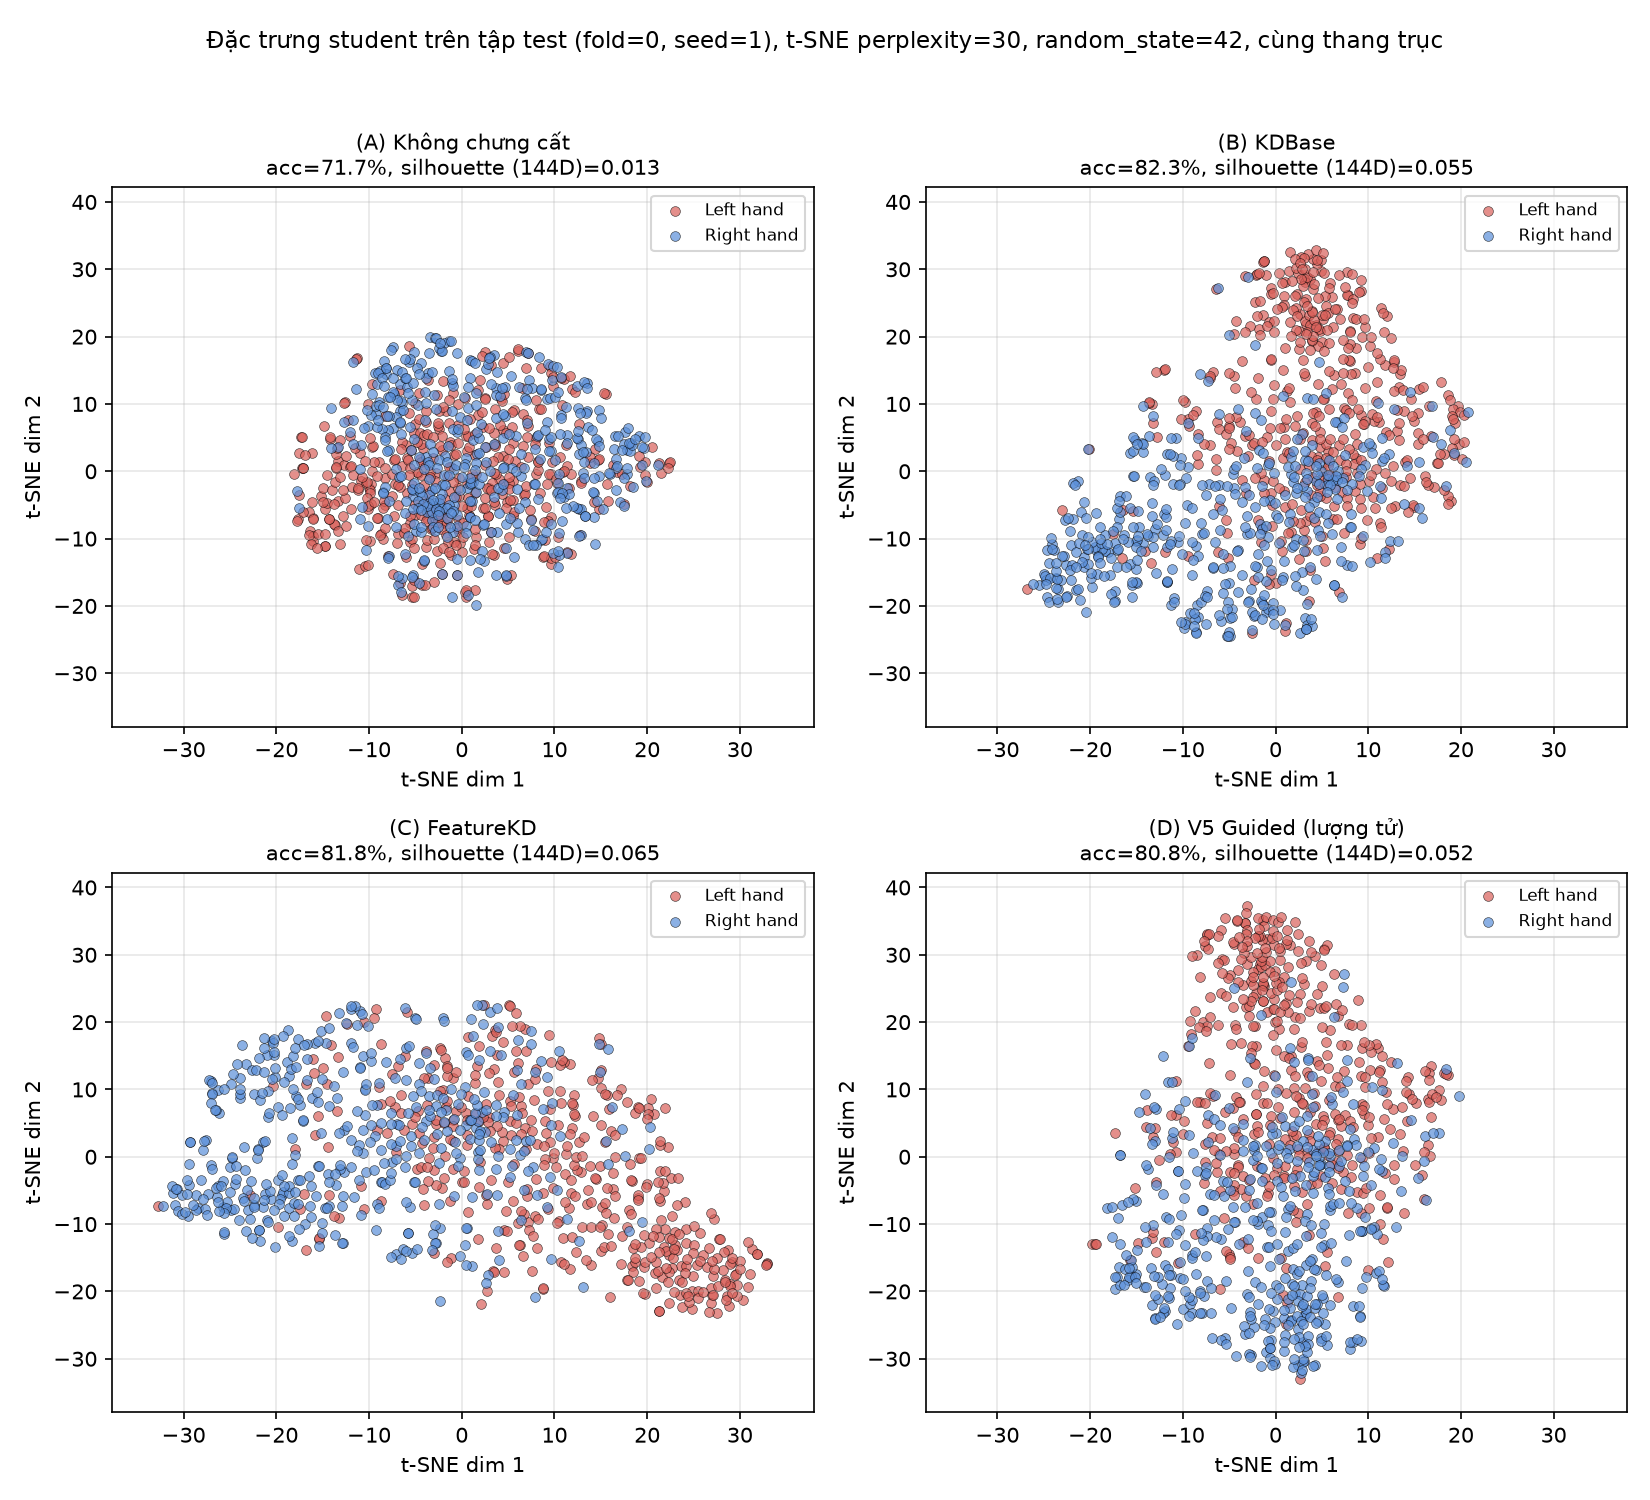
\includegraphics[width=\linewidth]{figs/image3.png}
\caption{Phân tích định tính không gian đặc trưng bằng trực quan hóa
t-SNE trên đặc trưng trung gian 144 chiều của student, trích trên tập
test tại epoch có độ chính xác thẩm định tốt nhất.}
\label{fig:tsne}
\end{figure}
\FloatBarrier

\section{Độ nhạy của cấu hình không chưng cất theo $\alpha$}
\label{app:alpha}

Cấu hình không chưng cất được huấn luyện thêm ở bốn giá trị $\alpha$ khác.
Bảng~\ref{tab:alphasweep} cho thấy độ chính xác tăng đơn điệu theo $\alpha$,
từ mức xấp xỉ ngẫu nhiên ở $\alpha=0$ (không có tín hiệu giám sát nào từ nhãn
thật) tới $74{,}93\%$ ở $\alpha=1{,}0$. Nếu tính mức cải thiện do chưng cất ở
$\alpha = 0{,}5$, student độc lập chỉ đạt $63{,}06\%$ và mức cải thiện lên tới
$18{,}43$ điểm phần trăm. Chênh lệch này không phản ánh hai ước lượng ngang
hàng của cùng một hiệu ứng. Nó phản ánh việc $\alpha = 0{,}5$ không cho cấu
hình không chưng cất đủ trọng số của số hạng mất mát duy nhất nó có.
$\alpha = 1{,}0$ nhất quán với nguyên tắc trọng số đầy đủ áp dụng cho mọi cấu
hình khác. Độ lệch chuẩn qua hạt giống cũng tăng mạnh khi $\alpha$ giảm, lên
5,03 điểm ở $\alpha = 0{,}5$.

\begin{table}[!htbp]
\centering
\caption{Độ nhạy của cấu hình không chưng cất theo hệ số $\alpha$
(PhysionetMI, 5 hạt giống $\times$ 5 fold).}
\label{tab:alphasweep}
\begin{tabular}{cc}
\toprule
$\boldsymbol{\alpha}$ & \textbf{Accuracy (\%)} \\
\midrule
0,00 & $49{,}89 \pm 0{,}34$ \\
0,25 & $51{,}73 \pm 2{,}68$ \\
0,50 & $63{,}06 \pm 5{,}03$ \\
0,75 & $71{,}45 \pm 3{,}74$ \\
1,00 (dùng cho baseline chính) & $\boldsymbol{74{,}93 \pm 2{,}30}$ \\
\bottomrule
\end{tabular}
\end{table}
\FloatBarrier

\section{Kết quả đầy đủ trên Cho2017}
\label{app:cho}

Bảy cấu hình dùng hàm nhân lượng tử (V1--V5 và hai biến thể $\beta$ của V5)
được huấn luyện với mạch lượng tử mô tả ở Mục~\ref{sec:qrd}. Sáu cấu hình cổ
điển không phụ thuộc mạch lượng tử nên giữ số liệu đã có.
Bảng~\ref{tab:cho2017} báo cáo độ chính xác của cả mười ba cấu hình. Mọi cấu
hình có chưng cất nằm trong khoảng 71,17\% đến 72,57\%. Ba cấu hình có
$p < 0{,}05$ so với KDBase là FeatureKD, nhân cosine và V5 Guided ở
$\beta = 0{,}01$. Hai cấu hình sau không có phép so sánh tương ứng trên
PhysionetMI nên chỉ được báo cáo.

\begin{table}[!htbp]
\centering
\caption{Kết quả trên Cho2017 (49 đối tượng, 5 hạt giống độc lập). $\Delta$, khoảng tin cậy 95\% và $d_z$ tính so với KDBase.}
\label{tab:cho2017}
\small
\begin{tabular}{lcccc}
\toprule
\textbf{Cấu hình} & \textbf{Accuracy (\%)} & $\boldsymbol{\Delta}$ \textbf{[CI 95\%]} & $\boldsymbol{p}$ & $\boldsymbol{d_z}$ \\
\midrule
No KD & $70{,}32 \pm 0{,}64$ & $-2{,}22$ $[-3{,}06; -1{,}39]$ & 0,0018 & $-3{,}30$ \\
KDBase & $72{,}54 \pm 0{,}21$ & --- & --- & --- \\
FeatureKD & $71{,}17 \pm 0{,}69$ & $-1{,}38$ $[-1{,}98; -0{,}77]$ & 0,0032 & $-2{,}83$ \\
RelationalKD & $72{,}57 \pm 0{,}42$ & $+0{,}03$ $[-0{,}38; +0{,}43]$ & 0,864 & $+0{,}08$ \\
\midrule
V1 Dense & $72{,}31 \pm 0{,}69$ & $-0{,}24$ $[-0{,}94; +0{,}47]$ & 0,405 & $-0{,}42$ \\
V2 Dense & $72{,}37 \pm 0{,}43$ & $-0{,}18$ $[-0{,}63; +0{,}28]$ & 0,343 & $-0{,}48$ \\
V3 Anchor & $72{,}03 \pm 0{,}63$ & $-0{,}51$ $[-1{,}20; +0{,}18]$ & 0,110 & $-0{,}92$ \\
V4 Anchor $+$ kNN & $72{,}28 \pm 0{,}56$ & $-0{,}26$ $[-0{,}71; +0{,}19]$ & 0,182 & $-0{,}72$ \\
V5 Guided & $72{,}41 \pm 0{,}65$ & $-0{,}13$ $[-0{,}83; +0{,}57]$ & 0,626 & $-0{,}24$ \\
V5 Guided ($\beta = 0{,}01$) & $72{,}17 \pm 0{,}38$ & $-0{,}37$ $[-0{,}63; -0{,}11]$ & 0,018 & $-1{,}74$ \\
V5 Guided ($\beta = 0{,}05$) & $72{,}36 \pm 0{,}27$ & $-0{,}19$ $[-0{,}42; +0{,}05]$ & 0,091 & $-0{,}99$ \\
\midrule
Nhân cosine & $72{,}13 \pm 0{,}30$ & $-0{,}41$ $[-0{,}76; -0{,}06]$ & 0,030 & $-1{,}47$ \\
Nhân RBF & $72{,}36 \pm 0{,}52$ & $-0{,}18$ $[-0{,}79; +0{,}42]$ & 0,452 & $-0{,}37$ \\
\bottomrule
\end{tabular}
\end{table}
\FloatBarrier

\section{Chi phí huấn luyện theo số qubit}
\label{app:qubit}

Một khảo sát sơ bộ đo thời gian huấn luyện theo số qubit
($n_{\text{qubits}} \in \{4, 8, 12, 16\}$, 1 fold, 3 epoch, giữ cố định mọi
siêu tham số khác) dùng V2 Dense. V2 và V5 có cùng chi phí đo được vì chọn cùng
số cặp mẫu cho hàm nhân, chỉ khác tiêu chí chọn. Số qubit chỉ ảnh hưởng tới chi
phí mỗi lần tính hàm nhân nên xu hướng đo trên V2 có cơ sở để suy rộng sang
các biến thể khác về chi phí chứ không về độ chính xác.
Bảng~\ref{tab:qubitcost} cho thấy chi phí tăng siêu tuyến tính. Bội số giữa
các mức liên tiếp (khoảng $2{,}8\times$, $1{,}8\times$ và $4{,}5\times$ cho mỗi
bước 4 qubit) thấp hơn nhiều mức $16\times$ mà mô phỏng statevector dự đoán cho riêng phần mạch. Điều này gợi ý rằng chi phí cố định (nạp dữ liệu, backbone cổ
điển, overhead của PennyLane) vẫn chiếm tỷ trọng đáng kể ở quy mô này. Ở
$n_{\text{qubits}}=16$, phép đo không hoàn tất 3 epoch trong 20 phút. Ước tính
một lượt đầy đủ ở mức này cần khoảng 65 giờ cho một cấu hình, vượt khả năng
của hạ tầng hiện có. Ở 8 và 12 qubit, độ chính xác đầy đủ được đo cho V2
Dense. Không cặp nào trong ba mức qubit khác biệt có ý nghĩa (kể cả 8 so với
12, $p=0{,}491$). Với $n=5$, kết quả này chỉ cho thấy chưa phát hiện được xu
hướng theo số qubit.

\begin{table}[!htbp]
\centering
\caption{Chi phí huấn luyện và độ chính xác theo số qubit (V2 Dense).
Thời gian/epoch đo ở khảo sát sơ bộ (1 fold $\times$ 3 epoch). Độ chính
xác đo đầy đủ (5 hạt giống $\times$ 5 fold $\times$ 30 epoch) cho
$n_{\text{qubits}} \le 12$.}
\label{tab:qubitcost}
\footnotesize
\begin{tabular}{ccccc}
\toprule
$\boldsymbol{n_{\text{qubits}}}$ & \textbf{Thời gian/epoch (s)} & \textbf{Bội số so mức trước} & \textbf{Accuracy (\%)} & $\boldsymbol{p}$ \textbf{(so $n=4$)} \\
\midrule
4  & $\approx 13{,}6$ & -- & $81{,}49 \pm 0{,}78$ & -- \\
8  & 36--40 & $\approx 2{,}8\times$ & $81{,}36 \pm 0{,}38$ & $0{,}691$ \\
12 & 67--71 & $\approx 1{,}8\times$ & $81{,}16 \pm 0{,}75$ & $0{,}332$ \\
16 & 308--315 & $\approx 4{,}5\times$ & không đo (không hoàn tất 3 epoch) & -- \\
\bottomrule
\end{tabular}
\end{table}
\FloatBarrier

\section{Chi tiết đo độ trễ}
\label{app:dotre}

\textbf{CPU máy chủ HPC.} Phép đo chạy trên node tính toán dùng chung của cụm HPC với CPU AMD EPYC
9224 (24 lõi mỗi socket, 2 socket, xung nhịp tối đa $\approx 3{,}7$ GHz).
Phép đo dùng 8 luồng theo số CPU được cấp phát mặc định cho tiến trình, với
PyTorch 2.7.1, nền BLAS Intel oneAPI MKL mặc định, độ chính xác float32 và
hệ điều hành Linux nhân 5.14 (Enterprise Linux 9). Cấu hình được xác
nhận trên cùng node dù không loại trừ khả năng bản vá hệ điều hành thay đổi
đôi chút giữa các lần đo. Giá trị 3,17 ms của student cùng bậc độ lớn với mức
2,95 ms của một triển khai EEGNet khác trên vi điều khiển siêu tiết kiệm năng
lượng \cite{wang2024mibminet}. Đây là hai kiến trúc, hai bộ dữ liệu và hai
loại phần cứng khác nhau nên sự tương đồng này không chứng minh điều kiện
triển khai tương đương. Thời gian suy luận trên vi điều khiển còn phụ thuộc
số MAC, RAM trung gian, precision, thư viện kernel và loại vi điều khiển. MAC
và activation đỉnh ở Bảng~\ref{tab:tre} được tính giải tích từ kiến trúc
EEGNet, không đo trên phần cứng.

\textbf{Raspberry Pi 4.} Phép đo dùng cùng giao thức như trên CPU máy chủ (200 lần suy luận sau 20
lần khởi động, batch bằng một, không cấu hình số luồng đặc biệt). Phép đo
được lặp 5 lần chạy độc lập và kiểm chứng lại bằng một lượt bổ sung, cho kết
quả nhất quán. Độ trễ của student dao động từ $11{,}7$ đến $15{,}0$ ms qua mọi
lần đo, ở $42{,}3^\circ$C, không bị giới hạn nhiệt, tần số CPU giữ ở mức tối đa 1800
MHz. Phép đo dùng trọng số khởi tạo ngẫu nhiên vì thời gian suy luận và bộ nhớ
chỉ phụ thuộc kiến trúc và kích thước tensor. RAM đỉnh của teacher
($251{,}63 \pm 0{,}11$ MiB) chỉ cao hơn student khoảng $4{,}1\%$ dù teacher có
gấp $6{,}3$ lần số tham số. Phần lớn RAM đo được đến từ overhead cố định của
trình thông dịch Python và runtime PyTorch. Đây là RAM của toàn bộ tiến trình, khác về bản chất với ước tính
$\approx 600$ KB activation thuần của student. Hai con số này không nên được
so trực tiếp.

\section{Hiệu ứng tối thiểu phát hiện được}
\label{app:mde}

Bảng~\ref{tab:mde} báo cáo hiệu ứng tối thiểu phát hiện được (MDE) ở công
suất 80\% cho từng phép so sánh trên PhysionetMI, với kiểm định $t$ ghép cặp
hai phía, $\alpha = 0{,}05$, $n = 5$ hạt giống, tính bằng phân phối $t$ không
trung tâm. Phân tích dùng độ lệch chuẩn chênh lệch ghép cặp quan sát được nên
là phân tích hậu nghiệm, không phải tính toán cỡ mẫu trước khi chạy. Với các
cơ chế có chưng cất, MDE nằm trong khoảng 0,65 đến 1,35 điểm phần trăm tùy độ
lệch chuẩn của từng cặp. Với
ba phép so sánh hàm nhân và V1 so V2, MDE từ 0,68 đến 0,87 điểm, đều lớn hơn
biên tương đương $\pm 0{,}5$ điểm. Thiết kế năm hạt giống do đó không đủ
công suất để phát hiện tin cậy một khác biệt cỡ biên tương đương, phù hợp với
kết luận chưa đủ dữ liệu ở Mục~\ref{sec:chuyensau}.

\begin{table}[!htbp]
\centering
\caption{Hiệu ứng tối thiểu phát hiện được ở công suất 80\% (PhysionetMI, phân tích hậu nghiệm). $\Delta$ quan sát và độ lệch chuẩn chênh lệch ghép cặp tính theo điểm phần trăm.}
\label{tab:mde}
\small
\begin{tabular}{lccc}
\toprule
\textbf{Phép so sánh} & $\boldsymbol{\Delta}$ \textbf{quan sát} & \textbf{SD chênh lệch} & \textbf{MDE 80\%} \\
\midrule
No KD so KDBase & $-6{,}56$ & 2{,}00 & 3{,}36 \\
FeatureKD so KDBase & $-1{,}44$ & 0{,}80 & 1{,}35 \\
RelationalKD so KDBase & $+0{,}12$ & 0{,}78 & 1{,}30 \\
V1 Dense so KDBase & $+0{,}41$ & 0{,}53 & 0{,}89 \\
V2 Dense so KDBase & $+0{,}00$ & 0{,}44 & 0{,}73 \\
V3 Anchor so KDBase & $-0{,}24$ & 0{,}51 & 0{,}86 \\
V4 Anchor $+$ kNN so KDBase & $-0{,}07$ & 0{,}50 & 0{,}85 \\
V5, nhân lượng tử so KDBase & $-0{,}37$ & 0{,}58 & 0{,}98 \\
V5, nhân cosine so KDBase & $+0{,}14$ & 0{,}56 & 0{,}94 \\
V5, nhân RBF so KDBase & $+0{,}13$ & 0{,}39 & 0{,}65 \\
\midrule
Lượng tử so cosine (V5) & $-0{,}50$ & 0{,}52 & 0{,}87 \\
Lượng tử so RBF (V5) & $-0{,}49$ & 0{,}42 & 0{,}71 \\
V1 so V2 & $+0{,}41$ & 0{,}40 & 0{,}68 \\
\bottomrule
\end{tabular}
\end{table}
\FloatBarrier

\section*{Lời cảm ơn}

Nội dung lời cảm ơn được tạm ẩn trong quá trình phản biện kín và sẽ
được bổ sung ở bản thảo cuối cùng sau khi bài được chấp nhận.

% \hypertarget{tuxe0i-liux1ec7u-tham-khux1ea3o}{%
